%% ===========================================================
%% 09_final_report.tex
%% Money and Success in Football
%% Sports Economics Seminar — Summer Semester 2026
%%
%% Compile with:  xelatex 09_final_report.tex  (twice for ToC/refs)
%%   or           pdflatex 09_final_report.tex
%% Figures live in ../outputs/ relative to this file.
%% ===========================================================
\documentclass[11pt, a4paper]{article}

%% ── Encoding & fonts ─────────────────────────────────────────
\usepackage[T1]{fontenc}
\usepackage[utf8]{inputenc}
\usepackage{microtype}

%% ── Page geometry ────────────────────────────────────────────
\usepackage[top=2.5cm, bottom=2.5cm, left=3cm, right=2.5cm,
            headheight=14pt]{geometry}

%% ── Maths ────────────────────────────────────────────────────
\usepackage{amsmath, amssymb}

%% ── Graphics ─────────────────────────────────────────────────
\usepackage{graphicx}
\graphicspath{{../outputs/}}
\usepackage{float}
\usepackage[labelfont=bf, labelsep=period,
            font=small, skip=4pt]{caption}

%% ── Tables ───────────────────────────────────────────────────
\usepackage{booktabs}
\usepackage{array}
\usepackage{colortbl}
\usepackage{multirow}
\usepackage{longtable}
\usepackage{makecell}

%% ── Colour palette ───────────────────────────────────────────
\usepackage[dvipsnames, table]{xcolor}
\definecolor{NavyBlue}{HTML}{1A2A4A}
\definecolor{Gold}{HTML}{F5A623}
\definecolor{SteelBlue}{HTML}{2C3E73}
\definecolor{ForestGreen}{HTML}{196F3D}
\definecolor{BrickRed}{HTML}{C0392B}
\definecolor{RowA}{HTML}{EBF5FB}
\definecolor{RowB}{HTML}{FEF9E7}
\definecolor{RowC}{HTML}{FDEDEC}
\definecolor{RowD}{HTML}{EAFAF1}

%% ── Callout boxes ────────────────────────────────────────────
\usepackage[most]{tcolorbox}

\tcbset{
  seminarbox/.style={
    enhanced, breakable,
    left=6pt, right=6pt, top=6pt, bottom=6pt,
    boxrule=0pt, leftrule=4pt,
    arc=2pt, outer arc=2pt,
    fonttitle=\small\bfseries,
    before skip=8pt, after skip=8pt
  }
}
\newtcolorbox{findingbox}[1][]{
  seminarbox,
  colback=RowB, colframe=Gold, #1
}
\newtcolorbox{alertbox}[1][]{
  seminarbox,
  colback=RowC, colframe=BrickRed, #1
}
\newtcolorbox{statbox}[1][]{
  seminarbox,
  colback=RowA, colframe=SteelBlue, #1
}
\newtcolorbox{successbox}[1][]{
  seminarbox,
  colback=RowD, colframe=ForestGreen, #1
}

%% ── Section styling ──────────────────────────────────────────
\usepackage{titlesec}
\titleformat{\section}{\large\bfseries\color{NavyBlue}}{\thesection}{0.8em}{}[\vspace{-2pt}\color{NavyBlue}\hrule\vspace{4pt}]
\titleformat{\subsection}{\normalsize\bfseries\color{SteelBlue}}{\thesubsection}{0.6em}{}
\titleformat{\subsubsection}{\normalsize\itshape\color{SteelBlue}}{\thesubsubsection}{0.5em}{}

%% ── Headers & footers ────────────────────────────────────────
\usepackage{fancyhdr}
\pagestyle{fancy}
\fancyhf{}
\fancyhead[L]{\small\color{NavyBlue}\textit{Money and Success in Football}}
\fancyhead[R]{\small\color{NavyBlue}Md.\ Muktadir --- Sports Economics Seminar 2026}
\fancyfoot[C]{\small\thepage}
\renewcommand{\headrulewidth}{0.4pt}

%% ── Hyperlinks ───────────────────────────────────────────────
\usepackage{hyperref}
\hypersetup{
  colorlinks = true,
  linkcolor  = NavyBlue,
  citecolor  = SteelBlue,
  urlcolor   = SteelBlue,
  pdftitle   = {Money and Success in Football},
  pdfauthor  = {Md. Muktadir}
}

%% ── Lists ────────────────────────────────────────────────────
\usepackage{enumitem}
\setlist{noitemsep, topsep=4pt}

%% ── Misc ─────────────────────────────────────────────────────
\usepackage{setspace}
\onehalfspacing
\usepackage{parskip}
\setlength{\parskip}{6pt}
\usepackage{lscape}

%% ── References ───────────────────────────────────────────────
\usepackage[numbers, sort&compress]{natbib}

%% ===========================================================
%%  DOCUMENT
%% ===========================================================
\begin{document}

%% ── Title page ───────────────────────────────────────────────
\begin{titlepage}
  \thispagestyle{empty}
  \vspace*{2cm}
  {\color{NavyBlue}\hrule height 2pt}
  \vspace{0.6cm}
  {\huge\bfseries\color{NavyBlue} Money and Success in Football}\\[0.4cm]
  {\large\color{SteelBlue} Does Financial Strength Predict League Position?}
  \vspace{0.4cm}
  {\color{NavyBlue}\hrule height 1pt}
  \vspace{1.2cm}

  \begin{tabular}{ll}
    \textbf{Author:}    & Md.\ Muktadir \\[3pt]
    \textbf{Contact:}   & \href{mailto:mdmuktadir0611@gmail.com}{mdmuktadir0611@gmail.com} \\[3pt]
    \textbf{Course:}    & Sports Economics Seminar \\[3pt]
    \textbf{Semester:}  & Summer 2026 \\[3pt]
    \textbf{Date:}      & June 2026 \\
  \end{tabular}

  \vspace{1.8cm}
  \begin{abstract}
    \noindent
    This study examines whether a football club's financial strength --- measured
    by its within-league-season squad market value rank --- predicts its final
    league standing. We analyse 975 team-season observations across the five major
    European leagues (Bundesliga, La Liga, Ligue~1, Premier League, Serie~A) from
    2015--16 through 2024--25. The Pearson correlation between Financial Rank
    and final league position is \(r = 0.813\) (\(p < 0.001\)), and a quadratic
    OLS model (Model~H) explains \(R^{2} = 0.671\) of all positional variation
    using a single predictor. Robustness checks confirm the quadratic specification
    outperforms all alternatives (lowest AIC = 5070.5), the relationship is
    identical across all five leagues (\(F_{4} = 1.17\), \(p = 0.324\)),
    and stable over the decade (\(F_{1} = 0.44\), \(p = 0.506\)). Of 50 league
    titles in the study period, 38 (76\,\%) were won by the financially wealthiest
    club; only four champions came from outside the financial top three. A logistic
    model predicts championship probability as a steep declining function of
    Financial Rank (McFadden \(R^{2} = 0.548\)). Leicester City 2015--16
    (Financial Rank~11, residual $-10.5$ positions, Cook's~$D = 0.187$)
    remains the sole genuine statistical outlier in ten years of European football.

    \medskip\noindent
    \textbf{Keywords:} football economics, squad market value, Financial Fair
    Play, sports analytics, regression, outlier analysis
  \end{abstract}

  \vfill
  {\small\color{gray}
    Data sources: ESPN FC (league standings), Transfermarkt (squad market values).\\
    Analysis: R~4.x with packages \texttt{dplyr}, \texttt{ggplot2}, \texttt{broom},
    \texttt{kableExtra}.}
\end{titlepage}

\clearpage
\tableofcontents
\clearpage

%% ===========================================================
\section{Executive Summary}
%% ===========================================================

\begin{statbox}
  \textbf{Scale of study:} 975 team-season observations spanning 5 major European
  leagues (Bundesliga, La Liga, Ligue~1, Premier League, Serie~A) over 10 complete
  seasons (2015--16 through 2024--25). Every club that completed a top-flight
  season appears once per season in the dataset.
\end{statbox}

\begin{findingbox}
  \textbf{Core finding:} The Pearson correlation between Financial Rank and final
  league position is \(\mathbf{r = 0.813}\) (Spearman \(\rho = 0.814\), both
  \(p < 0.001\)). The best-fitting model --- Model~H, which adds a quadratic term
  to Financial Rank --- explains \(\mathbf{R^{2} = 0.671}\) of all variation in
  final standings. Knowing only how wealthy a club is relative to its peers allows
  us to correctly explain \textbf{67\,\%} of where they finish.
\end{findingbox}

\begin{successbox}
  \textbf{Champions by financial rank:} 76\,\% of the 50 league titles in the study
  were won by the squad with the \textbf{highest market value} in their league that
  season (Financial Rank = 1). Only 4 champions came from outside the financial top
  three --- and only one of them (Leicester City 2015--16) qualifies as a genuine
  statistical outlier.
\end{successbox}

\begin{alertbox}
  \textbf{The one true exception:} Leicester City 2015--16 finished Financial
  Rank~11 in the Premier League yet won the title. The model predicted they would
  finish 11th; instead they came 1st. Their residual of \(\mathbf{-10.5}\)
  positions is the largest shock in the entire dataset and a once-in-a-generation
  event (\(3.2\) standard deviations below the mean).
\end{alertbox}

%% ===========================================================
\section{Introduction}
%% ===========================================================

\subsection{Why Does This Question Matter?}

The five major European football leagues --- the English Premier League, Spanish
La~Liga, German Bundesliga, Italian Serie~A, and French Ligue~1 --- collectively
generate over \EUR{}18 billion in annual revenue, with squad transfer spending
exceeding \EUR{}12 billion in recent seasons. With this much money flowing through
the sport, a natural and important question arises: \textbf{does financial
investment actually buy success, or can a well-organised, under-funded club
systematically compete at the top level?}

This question extends well beyond football. It has direct implications for:

\begin{itemize}
  \item \textbf{Competitive balance policy} --- UEFA introduced Financial Fair Play
        precisely to prevent the wealthiest clubs from buying their way to
        dominance. If money truly determines outcomes, these policies become
        even more critical.
  \item \textbf{Fan engagement} --- If leagues are financially predetermined,
        the drama of competition is diminished for supporters of smaller clubs.
  \item \textbf{Sports economics theory} --- Understanding how resource endowments
        translate to tournament outcomes informs models across all competitive
        sports~\citep{Szymanski1999, Frick2007}.
\end{itemize}

\subsection{Research Questions}

This study addresses three interrelated questions using ten years of data:

\begin{enumerate}
  \item \textbf{Direction and strength:} Is there a statistically significant
        relationship between a squad's financial rank within its league and its
        final position? How strong is that relationship?
  \item \textbf{Model form:} Does a simple linear relationship capture the data,
        or is there a non-linear pattern? Does the relationship differ across
        leagues or change over time?
  \item \textbf{Exceptions:} Which clubs defy the financial hierarchy, and how
        statistically unusual are they?
\end{enumerate}

\subsection{Contribution}

Previous research~\citep{Szymanski1999, Frick2007} has shown that wage bills and
transfer spending predict league success. This study makes two additional
contributions. First, instead of raw market values, we use a
\textbf{within-league financial rank} --- which club was the $n$-th wealthiest
in their specific league that season. This removes the scale problem: a \EUR{}300M
squad is the richest in Ligue~1 but the fifth-richest in the Premier League. By
ranking within leagues we pool all five leagues and make fair comparisons. Second,
we introduce a \textbf{residual-based outlier framework} to systematically identify
and quantify clubs that dramatically beat or missed their financial prediction.

%% ===========================================================
\section{Data}
%% ===========================================================

\subsection{Sources and Construction}

Our dataset was assembled from two sources:

\begin{itemize}
  \item \textbf{ESPN FC} provided final league standings (league position) for all
        five leagues across the 2015--16 through 2024--25 seasons.
  \item \textbf{Transfermarkt} provided squad market values --- the estimated total
        transfer-market worth of all players in each squad --- at the start of each
        season.
\end{itemize}

After merging and removing rows with missing values on key variables, the clean
dataset contains \textbf{975 team-season observations}. Every team that played a
full season in one of the five leagues during the study period appears once per
season.

\subsection{Variable Definitions}

\begin{table}[H]
  \centering
  \small
  \caption{Variable definitions.}
  \label{tab:vardefs}
  \begin{tabular}{>{\ttfamily}p{3.6cm} p{1.4cm} p{1.6cm} p{7.2cm}}
    \toprule
    \rowcolor{NavyBlue}
    \color{white}\textbf{Variable} &
    \color{white}\textbf{Type} &
    \color{white}\textbf{Range} &
    \color{white}\textbf{Description} \\
    \midrule
    League\_Position    & Integer      & 1--20     & Final league standing; 1 = champion, higher = worse \\
    \rowcolor{RowA}
    Financial\_Rank (FR) & Integer     & 1--20     & Squad rank by market value within league-season; 1 = richest \\
    Market\_Value\_M\_EUR & Numeric    & 10--3300+ & Total squad value in millions of euros (Transfermarkt) \\
    \rowcolor{RowA}
    Normalized\_Value   & Numeric      & 0--1      & Market value normalised within league-season \\
    Log\_Normalized\_Value & Numeric   & $-\infty$--0 & Natural log of Normalized\_Value \\
    \rowcolor{RowA}
    Champion\_bin       & Binary (0/1) & 0 or 1   & 1 if the team won the league title, 0 otherwise \\
    Season\_Index       & Integer      & 1--10     & Season counter: 1 = 2015--16, 10 = 2024--25 \\
    \bottomrule
  \end{tabular}
\end{table}

\subsection{The Key Design Choice: Financial Rank over Raw Market Value}

Using Financial Rank (FR) rather than the raw \EUR{}-value is crucial for a
multi-league analysis. Consider: a squad worth \EUR{}300M is the \emph{richest}
in Ligue~1 but only the \emph{fifth-richest} in the Premier League. If we used
raw \EUR{}-values and pooled all leagues, we would be comparing apples to oranges.
By ranking each squad within its own league-season, we create a fair, scale-free
measure. FR\,=\,1 always means ``the wealthiest club in this league this season,''
regardless of whether that squad is worth \EUR{}600M or \EUR{}150M.

\subsection{Descriptive Statistics}

Table~\ref{tab:desc} summarises the key characteristics of the dataset by league.

\begin{table}[H]
  \centering
  \small
  \caption{Sample size and descriptive statistics by league.}
  \label{tab:desc}
  \begin{tabular}{l r r r r r r}
    \toprule
    \rowcolor{NavyBlue}
    \color{white}\textbf{Group} &
    \color{white}\textbf{N} &
    \color{white}\textbf{Mean Pos.} &
    \color{white}\textbf{SD Pos.} &
    \color{white}\textbf{Mean MV (M\EUR{})} &
    \color{white}\textbf{SD MV (M\EUR{})} &
    \color{white}\textbf{Pearson $r$} \\
    \midrule
    \rowcolor{RowA}
    \textbf{All leagues} & \textbf{975} & \textbf{10.27} & \textbf{5.66}
      & \textbf{277.9} & \textbf{254.4} & \textbf{0.813} \\
    Bundesliga      & 180 & 9.50  & 5.20 & 237.2 & 205.6 & 0.783 \\
    La Liga         & 200 & 10.50 & 5.78 & 256.7 & 269.4 & 0.787 \\
    Ligue 1         & 196 & 10.32 & 5.69 & 184.7 & 193.9 & 0.791 \\
    Premier League  & 200 & 10.50 & 5.78 & 458.0 & 303.5 & 0.801 \\
    Serie A         & 199 & 10.47 & 5.78 & 246.7 & 182.4 & 0.889 \\
    \bottomrule
  \end{tabular}
  \medskip

  \noindent\small Note: Mean Position and SD Position refer to final league
  standing (1 = champion). Pearson $r$ is the correlation between Financial Rank
  and final position; all correlations are statistically significant at $p < 0.001$.
\end{table}

%% ===========================================================
\section{Step 1 --- First Look: Does Money Relate to Success?}
%% ===========================================================

\subsection{The Main Scatter Plot}

\begin{figure}[H]
  \centering
  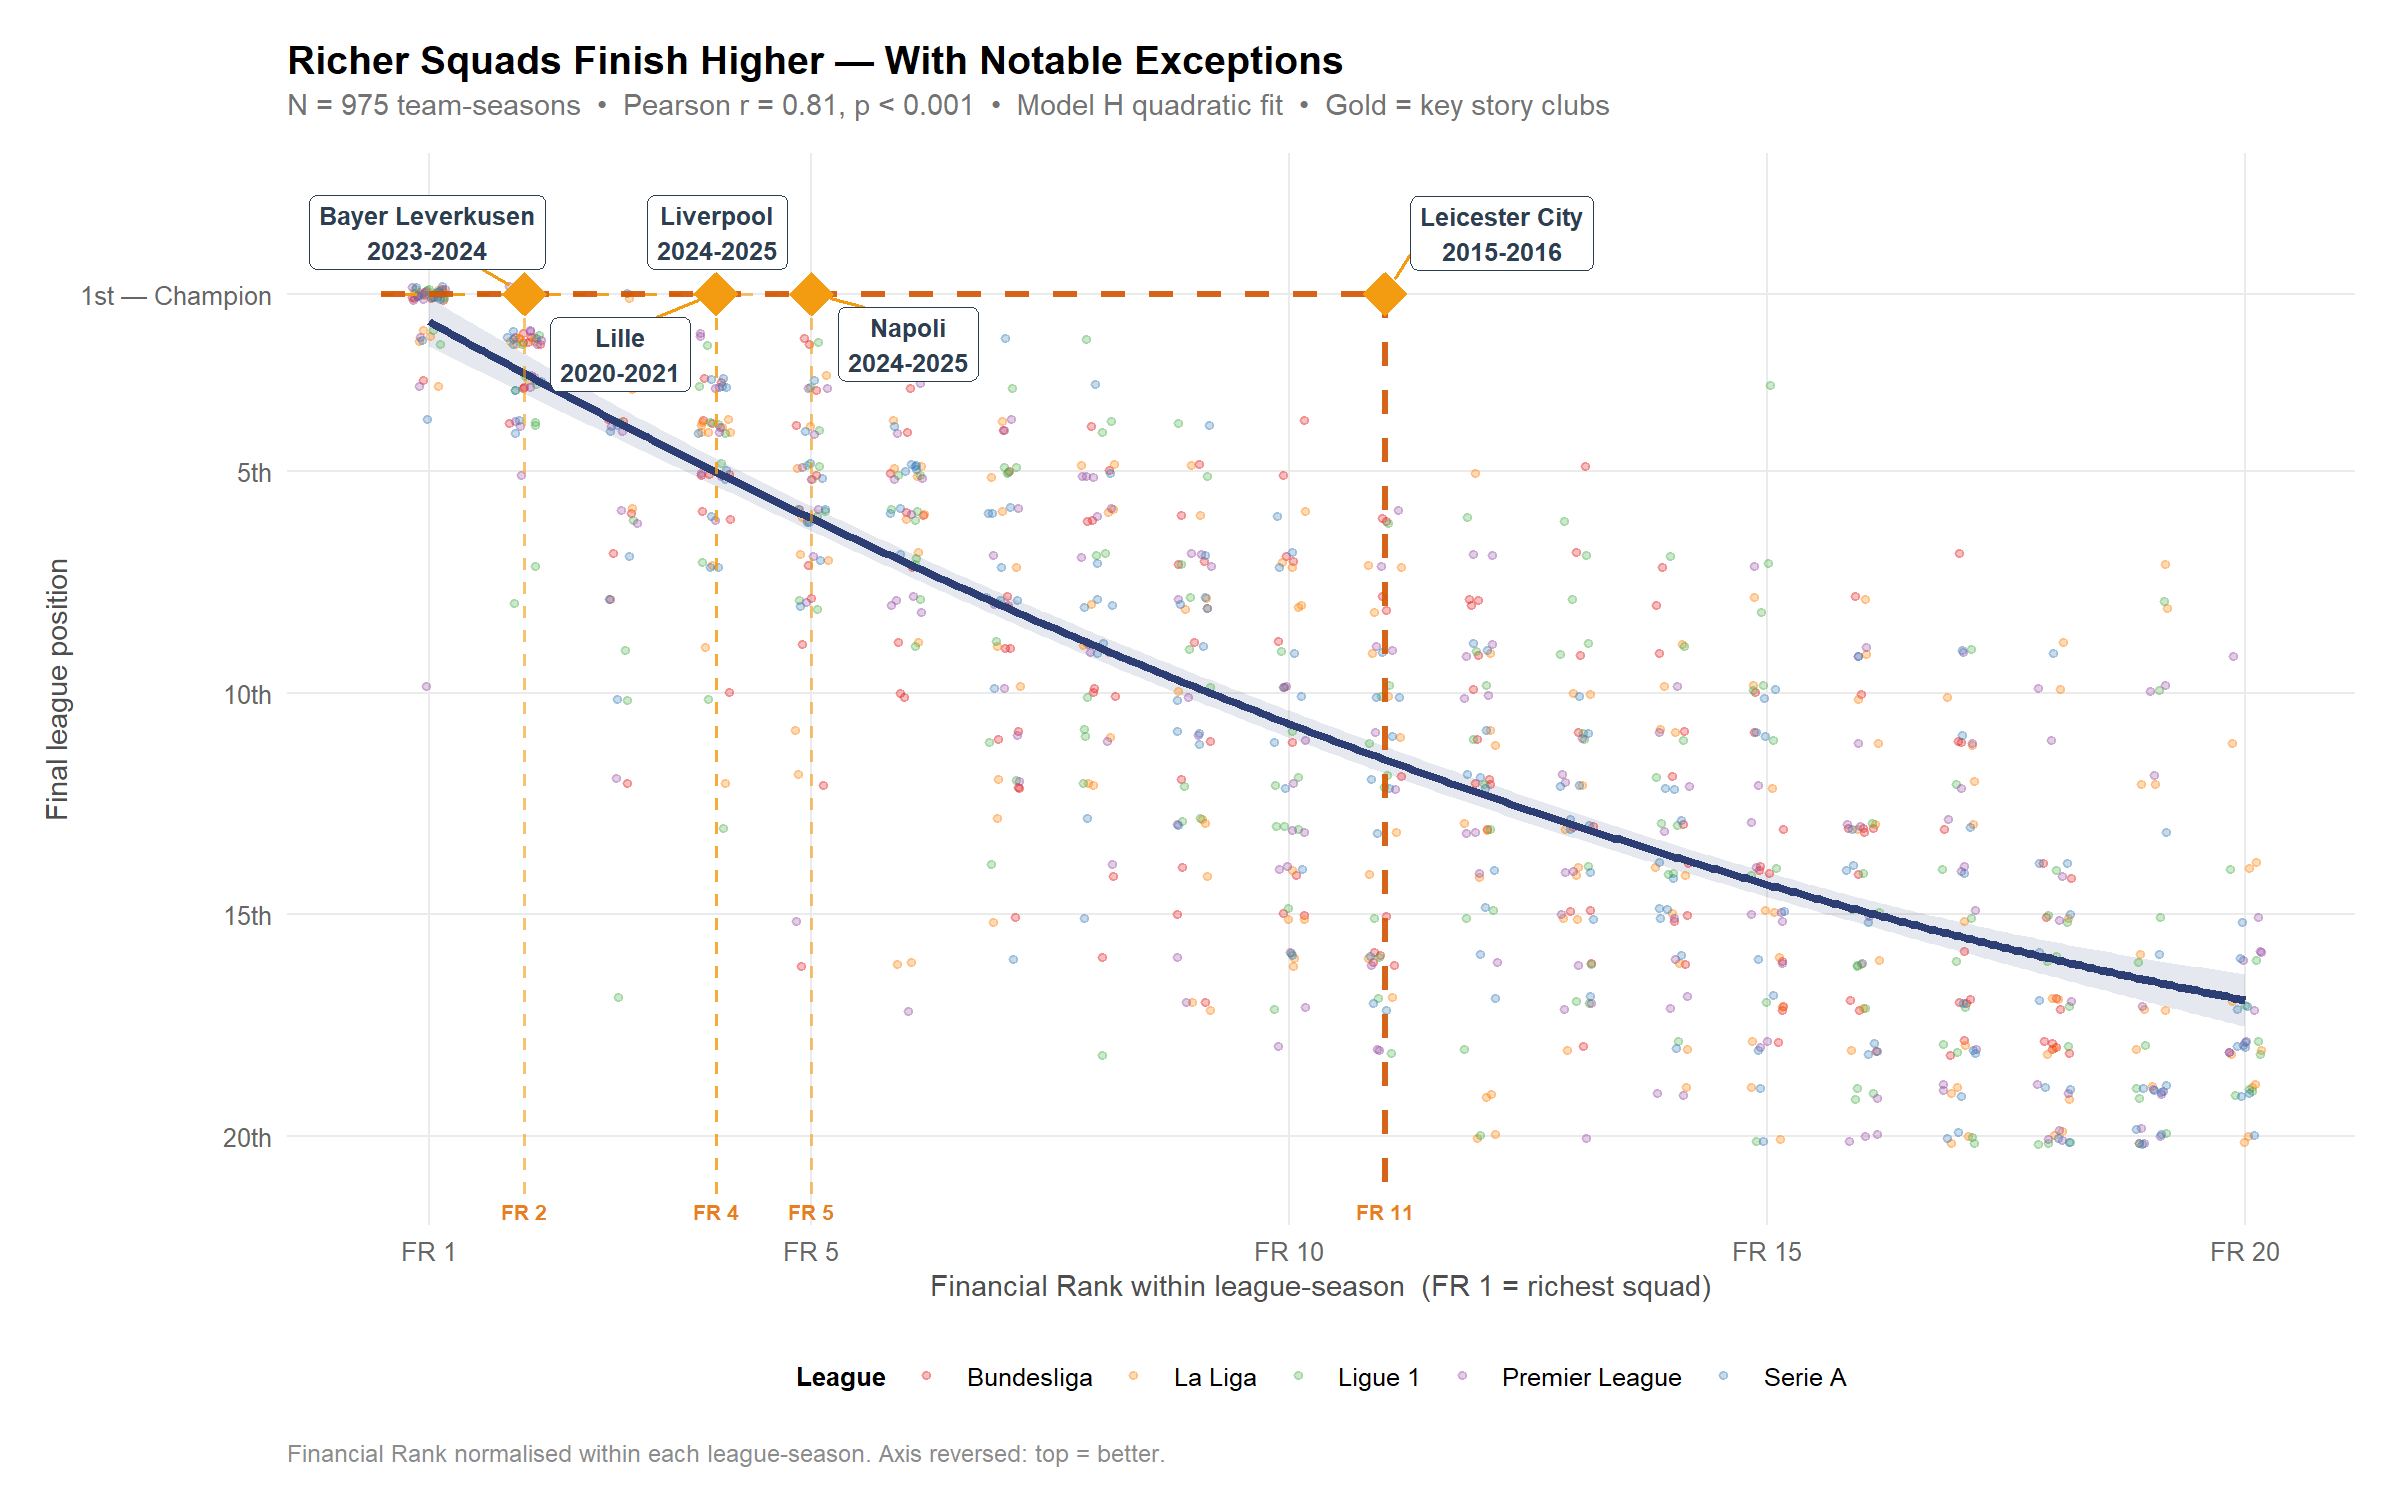
\includegraphics[width=0.95\linewidth, keepaspectratio]{33_scatter_story.png}
  \caption{Financial Rank vs.\ Final League Position for all 975 team-seasons.
    Each dot represents one team in one season, coloured by league. The dark
    fitted curve (with shaded 95\,\% confidence band) comes from Model~H
    (quadratic). The $y$-axis is reversed so that 1st place is at the top.}
  \label{fig:scatter}
\end{figure}

The downward-sloping pattern in Figure~\ref{fig:scatter} is immediately clear.
Clubs with Financial Rank 1 or 2 cluster near the top of their league, while
clubs with Financial Rank 15+ cluster near the bottom. The Pearson correlation
is \(\mathbf{r = 0.813}\) and the Spearman rank correlation is
\(\boldsymbol{\rho} = 0.814\) (both \(p < 0.001\), \(N = 975\)). A correlation
above 0.8 is considered very strong in social science contexts, and here we
achieve it with a single variable.

\subsection{Is the Relationship the Same in Every League?}

\begin{figure}[H]
  \centering
  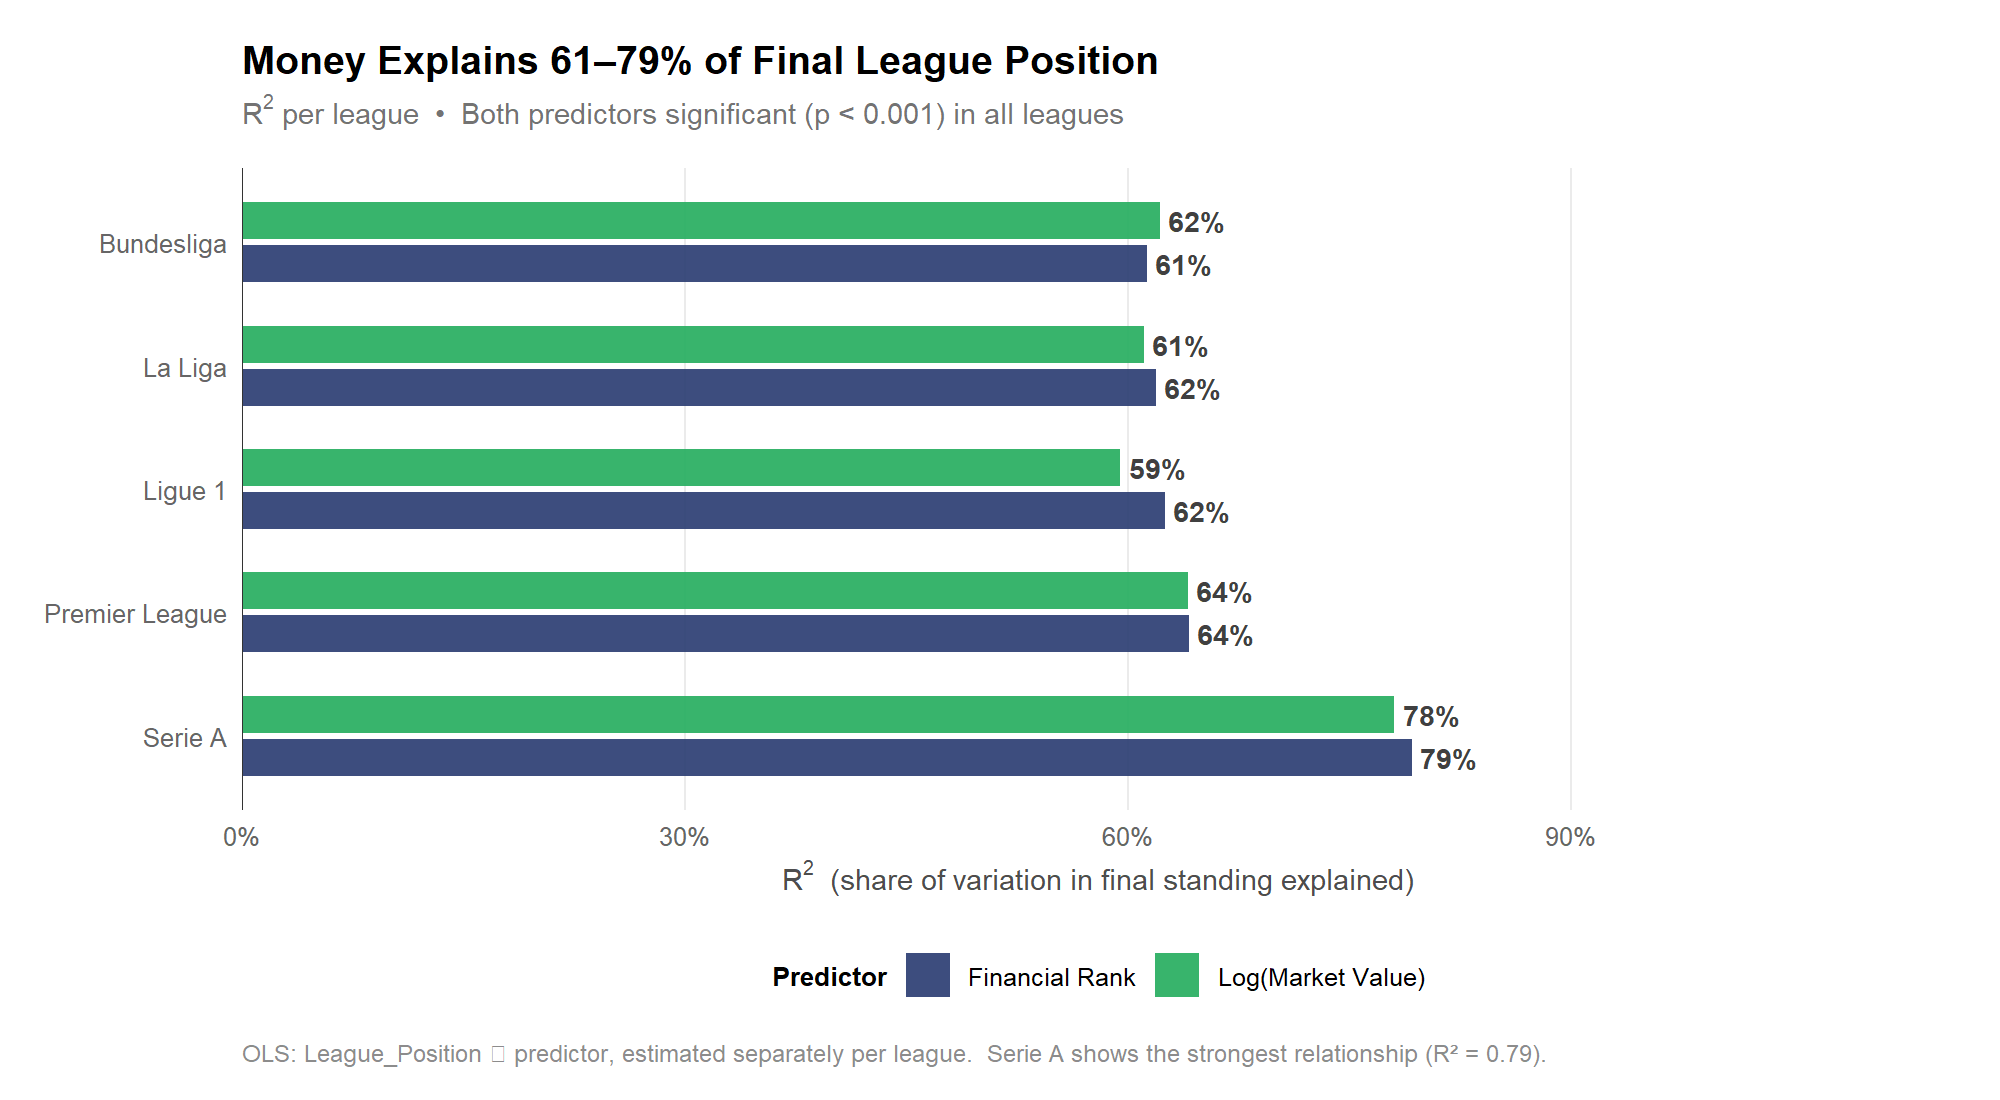
\includegraphics[width=0.90\linewidth, keepaspectratio]{32_league_r2_bars.png}
  \caption{$R^{2}$ (variance explained in final position by Financial Rank)
    broken down by league. Financial Rank alone explains 61--79\,\% of final
    standings, with Serie~A showing the strongest relationship ($R^{2} = 0.791$).}
  \label{fig:leaguer2}
\end{figure}

\begin{table}[H]
  \centering
  \small
  \caption{League-level correlation and simple regression results (response: League Position).}
  \label{tab:leaguecorr}
  \begin{tabular}{l r r r r r}
    \toprule
    \rowcolor{NavyBlue}
    \color{white}\textbf{League} &
    \color{white}\textbf{N} &
    \color{white}\textbf{Pearson $r$} &
    \color{white}\textbf{Spearman $\rho$} &
    \color{white}\textbf{$R^{2}$(FR)} &
    \color{white}\textbf{$\hat{\beta}$(FR)} \\
    \midrule
    Bundesliga      & 180 & 0.783 & 0.783 & 0.613 & 0.783 \\
    \rowcolor{RowA}
    La Liga         & 200 & 0.787 & 0.787 & 0.619 & 0.787 \\
    Ligue 1         & 196 & 0.791 & 0.791 & 0.625 & 0.791 \\
    \rowcolor{RowA}
    Premier League  & 200 & 0.801 & 0.801 & 0.641 & 0.800 \\
    \rowcolor{RowB}
    \textbf{Serie A} & \textbf{199} & \textbf{0.889} & \textbf{0.890}
      & \textbf{0.791} & \textbf{0.889} \\
    \bottomrule
  \end{tabular}
\end{table}

\begin{findingbox}
  \textbf{League-by-league finding:} Every single league displays a strong and
  statistically significant relationship between Financial Rank and final position.
  Serie~A shows the highest correlation ($r = 0.889$, $R^{2} = 0.791$), meaning
  that in Italy, financial rank almost perfectly determines where you finish.
  The Premier League ($r = 0.801$) and Bundesliga also show very strong
  relationships. Even the weakest correlation (Bundesliga, $R^{2} = 0.613$)
  remains extremely strong by any academic standard. This rules out the
  possibility that the pooled result is driven by one unusual league.
\end{findingbox}

%% ===========================================================
\section{Step 2 --- Building the Best Predictive Model}
%% ===========================================================

\subsection{Model Specifications}

We fit a series of OLS regression models, starting simple and progressively
adding complexity, then compare via AIC (Akaike Information Criterion). We also
fit a logistic regression for championship probability.

\begin{table}[H]
  \centering
  \small
  \caption{Model comparison. ($*$) = preferred specification (lowest AIC among OLS models). Model~E reports McFadden pseudo-$R^2$; Adj.~$R^2$ and BIC are not defined for logit.}
  \label{tab:modelcomp}
  \begin{tabular}{l p{5.5cm} r r r r}
    \toprule
    \rowcolor{NavyBlue}
    \color{white}\textbf{Model} &
    \color{white}\textbf{Formula} &
    \color{white}\textbf{$R^{2}$} &
    \color{white}\textbf{Adj.~$R^{2}$} &
    \color{white}\textbf{AIC} &
    \color{white}\textbf{BIC} \\
    \midrule
    A  & FR                               & 0.660 & 0.660 & 5099.8 & 5114.5 \\
    \rowcolor{RowA}
    B  & FR + League FE                   & 0.660 & 0.659 & 5107.4 & 5141.5 \\
    C  & Log(MV)                          & 0.533 & 0.532 & 5410.6 & 5425.2 \\
    \rowcolor{RowA}
    D  & Log(MV) + League + Season        & 0.641 & 0.638 & 5164.3 & 5203.3 \\
    G  & FR $\times$ League               & 0.662 & 0.659 & 5110.7 & 5164.4 \\
    \rowcolor{RowB}
    \textbf{H}$^*$ & \textbf{FR + FR}$^{\mathbf{2}}$
      & \textbf{0.671} & \textbf{0.670} & \textbf{5070.5} & \textbf{5090.1} \\
    \rowcolor{RowA}
    I  & FR + FR$^{2}$ + FR$^{3}$        & 0.671 & 0.670 & 5072.3 & 5096.7 \\
    J  & Log(FR)                          & 0.626 & 0.625 & 5194.0 & 5208.6 \\
    M  & $\sqrt{\text{FR}}$               & 0.669 & 0.668 & 5075.5 & 5090.2 \\
    \midrule
    E  & Champion $\sim$ FR (Logit)       & 0.548$^{\dagger}$ & --- & 182.4 & --- \\
    \bottomrule
  \end{tabular}
  \medskip

  \noindent\small $^{\dagger}$ McFadden pseudo-$R^{2}$.
  H2 (FR + FR$^2$ + League, AIC = 5077.3), H3 (FR + FR$^2$ + Season, AIC = 5072.5),
  and H4 (FR + FR$^2$ + League + Season, AIC = 5079.3) are also tested but all have
  higher AIC than Model~H; see Section~\ref{sec:robustness}.
\end{table}

\begin{findingbox}
  \textbf{Model H wins decisively.} The highlighted row (Model~H: League\_Position
  = $\alpha + \beta_1 \cdot \text{FR} + \beta_2 \cdot \text{FR}^2$) achieves the
  lowest AIC of any OLS model (5070.5). Compared to the simple linear baseline
  (Model~A, AIC = 5099.8), adding just one extra term (FR$^2$) reduces AIC by
  29.3~points. Model~I adds a cubic term but does not further improve fit
  (AIC~=~5072.3, cubic $F$-test: $F_{1} = 0.20$, $p = 0.653$). The quadratic
  specification is both statistically optimal and theoretically motivated by the
  principle of diminishing returns to financial advantage.
\end{findingbox}

\subsection{Model H Coefficients}

\begin{table}[H]
  \centering
  \small
  \caption{Model~H coefficient estimates. Response: League Position (1 = champion).
    $N = 975$, $R^{2} = 0.671$, Adj.~$R^{2} = 0.670$, AIC = 5070.5.}
  \label{tab:modelHcoefs}
  \begin{tabular}{l r r r l p{4.0cm}}
    \toprule
    \rowcolor{NavyBlue}
    \color{white}\textbf{Term} &
    \color{white}\textbf{Estimate} &
    \color{white}\textbf{Std.\ Error} &
    \color{white}\textbf{$t$-value} &
    \color{white}\textbf{$p$-value} &
    \color{white}\textbf{95\,\% CI} \\
    \midrule
    Intercept ($\alpha$)        & 0.4189  & 0.3442 &  1.217 & 0.224 & $[-0.256,\ 1.094]$ \\
    \rowcolor{RowA}
    Financial Rank ($\beta_1$)  & 1.2305  & 0.0765 & 16.083 & $< 0.001$ & $[1.081,\ 1.380]$ \\
    FR$^{2}$ ($\beta_2$)        & $-0.0202$ & 0.0036 & $-5.631$ & $< 0.001$ & $[-0.027,\ -0.013]$ \\
    \bottomrule
  \end{tabular}
\end{table}

\subsubsection{Interpreting the Coefficients}

\begin{itemize}
  \item \textbf{Intercept ($\alpha \approx 0.42$):} Anchors the curve at FR~=~0;
        no direct real-world interpretation.
  \item \textbf{$\beta_1 \approx 1.231$ (Financial Rank):} Each one-step increase
        in Financial Rank worsens the predicted final position by approximately
        \textbf{1.23~places} at the top of the hierarchy (FR~1\,\textrightarrow\,2).
  \item \textbf{$\beta_2 \approx -0.0202$ (FR$^2$):} The negative quadratic
        coefficient introduces \textbf{diminishing returns} at the bottom of the
        table. The marginal positional penalty of dropping one rank is:
        \begin{align*}
          \text{at FR} = 1{:} &\quad 1.231 - 2(0.0202)(1) \approx 1.19\ \text{positions/rank} \\
          \text{at FR} = 15{:} &\quad 1.231 - 2(0.0202)(15) \approx 0.63\ \text{positions/rank}
        \end{align*}
        In plain terms: the gap between the richest and second-richest club is
        nearly twice as large as the gap between the 15th and 16th richest.
  \item \textbf{$R^{2} = 0.671$:} Together, the linear and quadratic FR terms explain
        \textbf{67.1\,\%} of all variation in final league position across 975
        team-seasons --- using just one predictor variable.
\end{itemize}

\subsection{Visualising the Quadratic Fit}

\begin{figure}[H]
  \centering
  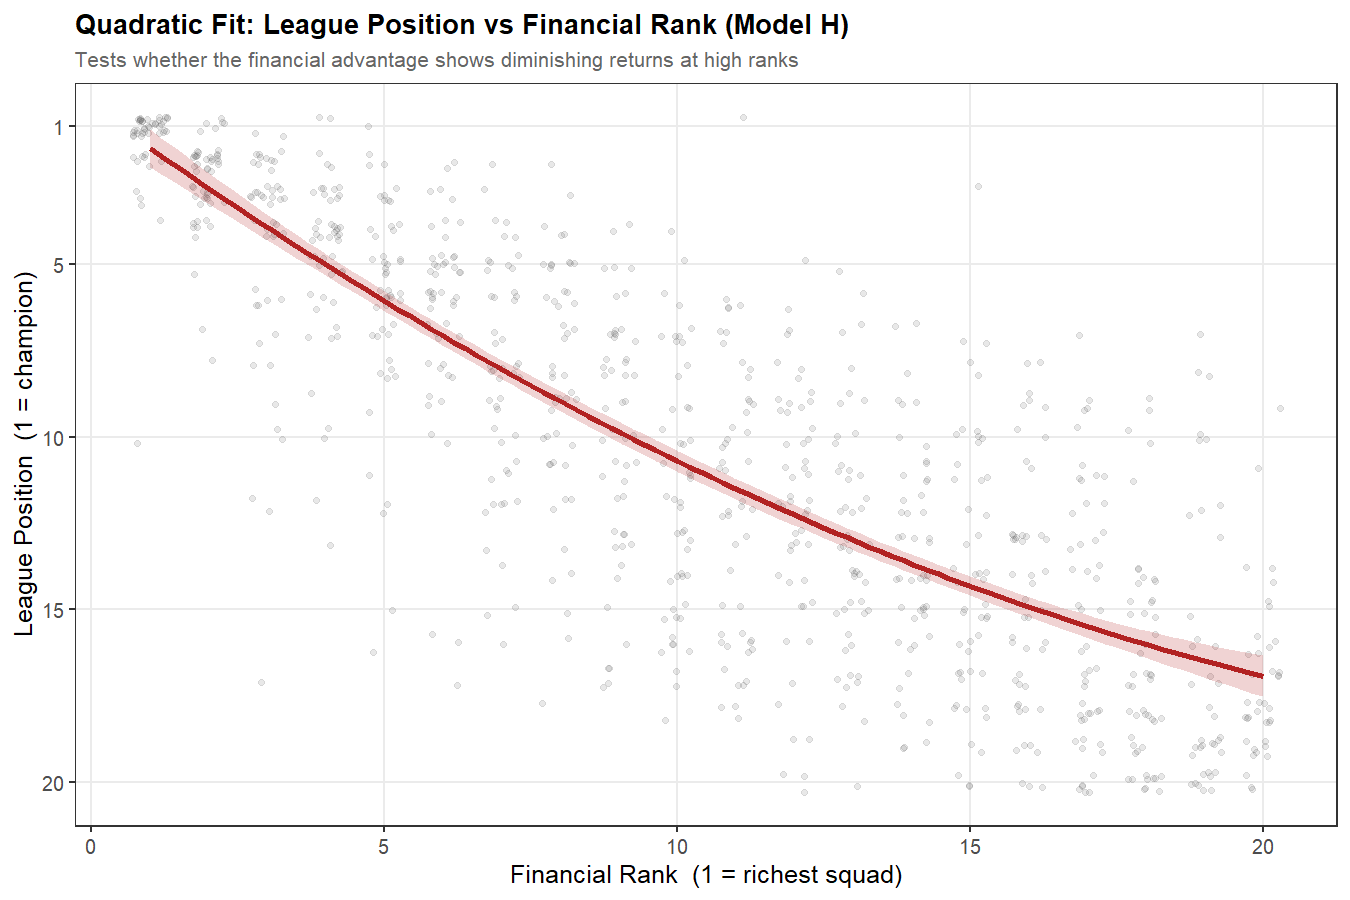
\includegraphics[width=0.92\linewidth, keepaspectratio]{21_quadratic_fit_plot.png}
  \caption{Model~H predicted league position as a function of Financial Rank,
    with 95\,\% confidence interval. The $y$-axis is reversed: lower position
    number = better finish. The curve bends rightward, reflecting diminishing
    returns at the bottom of the financial hierarchy.}
  \label{fig:quadfit}
\end{figure}

Figure~\ref{fig:quadfit} shows the predicted positions: a club ranked 1st
financially is predicted to finish around 2nd place; at FR\,=\,5, the model
predicts 5th--6th; at FR\,=\,10, approximately 11th; at FR\,=\,20, around
16th--17th (not last, due to diminishing returns).

%% ===========================================================
\section{Step 3 --- Can We Predict Who Wins the Title?}
\label{sec:logistic}
%% ===========================================================

\subsection{Championship Probability: Logistic Regression}

Model~E uses logistic regression to predict the binary outcome ``won the league
title'' as a function of Financial Rank:
\[
  \log\!\left(\frac{P(\text{Champion})}{1 - P(\text{Champion})}\right)
  = \alpha + \beta_{\text{FR}} \cdot \text{FR}
\]

\begin{table}[H]
  \centering
  \small
  \caption{Logistic Model~E coefficients. Response: Champion (1/0).
    McFadden $R^{2} = 0.548$, AIC = 182.4, $N = 975$.}
  \label{tab:logitcoefs}
  \begin{tabular}{l r r r l r}
    \toprule
    \rowcolor{NavyBlue}
    \color{white}\textbf{Term} &
    \color{white}\textbf{Log-Odds} &
    \color{white}\textbf{Std.\ Error} &
    \color{white}\textbf{$z$-value} &
    \color{white}\textbf{$p$-value} &
    \color{white}\textbf{Odds Ratio} \\
    \midrule
    Intercept ($\alpha$)          &  1.642 & 0.403 &  4.070 & $< 0.001$ & 5.165 \\
    \rowcolor{RowA}
    Financial Rank ($\beta$)      & $-1.298$ & 0.190 & $-6.834$ & $< 0.001$ & 0.273 \\
    \bottomrule
  \end{tabular}
\end{table}

The estimated $\beta = -1.298$ means each one-step increase in Financial Rank
\textbf{multiplies the odds of winning the title by} $e^{-1.298} = 0.273$ --- a
\textbf{72.7\,\% reduction in championship odds} per rank step. Moving from
FR\,1 to FR\,3 reduces odds by over 92\,\%.

\subsection{The Championship Probability Curve}

\begin{figure}[H]
  \centering
  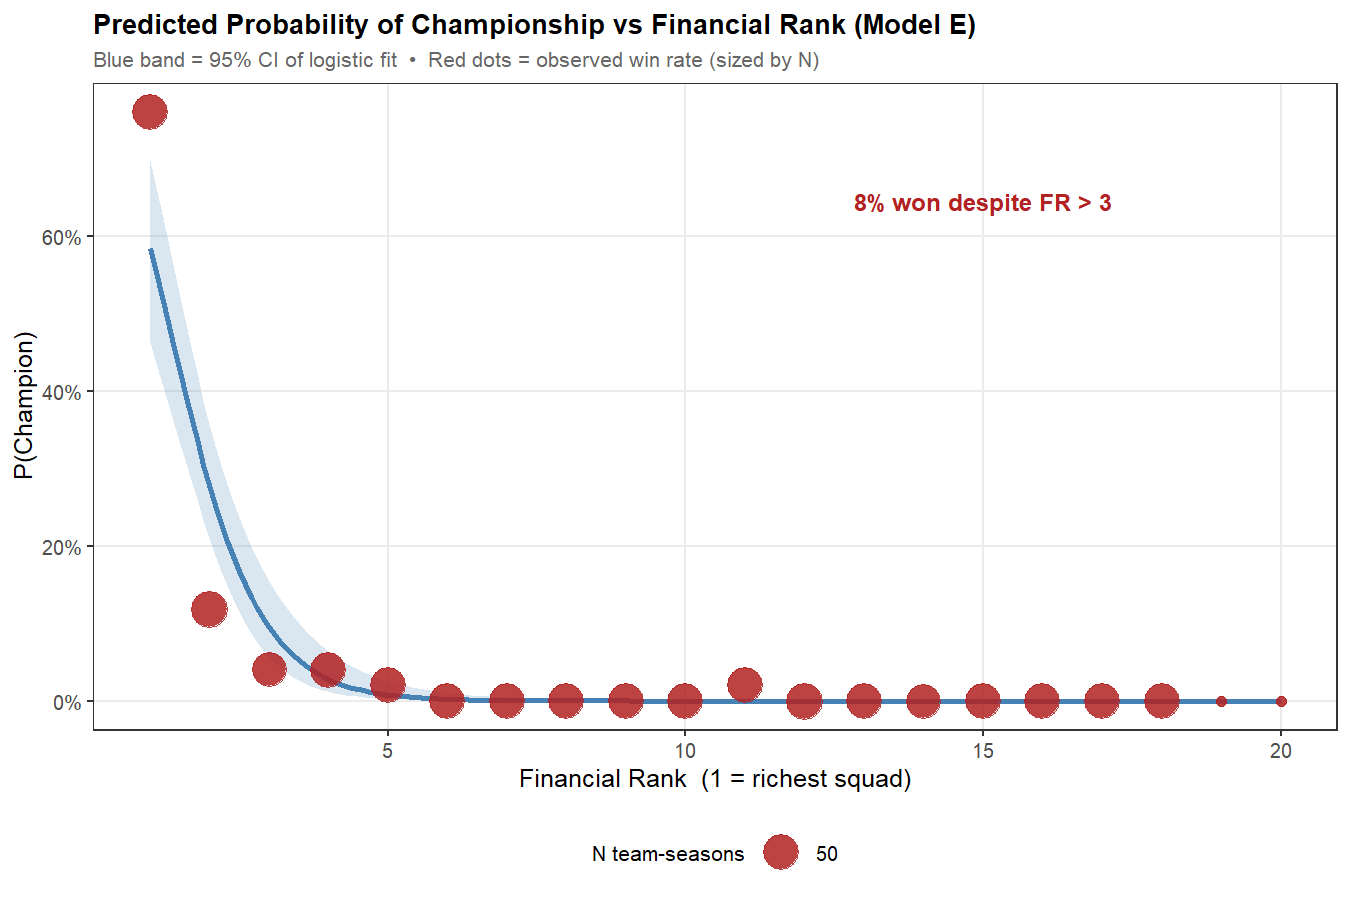
\includegraphics[width=0.92\linewidth, keepaspectratio]{12_champion_probability_curve.png}
  \caption{Predicted probability of winning the league title as a function of
    Financial Rank (Logistic Model~E). The richest squad (FR~=~1) has a predicted
    championship probability of 58.5\,\%; probability drops rapidly and is
    essentially zero by FR~=~8.}
  \label{fig:champprob}
\end{figure}

\begin{table}[H]
  \centering
  \small
  \caption{Predicted championship probabilities at key FR values (Model~E).}
  \label{tab:probfr}
  \begin{tabular}{c r}
    \toprule
    \rowcolor{NavyBlue}
    \color{white}\textbf{Financial Rank} &
    \color{white}\textbf{$P$(Champion)} \\
    \midrule
    \rowcolor{RowB}
    \textbf{1} & \textbf{58.5\,\%} \\
    2 &  28.0\,\% \\
    3 &  10.7\,\% \\
    4 &   3.9\,\% \\
    5 &   1.3\,\% \\
    8 &   $< 0.1$\,\% \\
    11 (Leicester 2015--16) & $\approx 0.001$\,\% \\
    \bottomrule
  \end{tabular}
\end{table}

\begin{statbox}
  \textbf{Practical interpretation:} The richest club in a league has a predicted
  championship probability of 58.5\,\% --- roughly 11 times higher than a random
  club (baseline 5.1\,\% per club in a 20-team league). By FR\,=\,5 the probability
  has fallen below 1.5\,\%. Leicester City's title in 2015--16 at FR\,=\,11 had
  a model-predicted probability of approximately 0.001\,\%. Football is inherently
  random, but the model captures a powerful structural advantage for wealthy clubs.
\end{statbox}

%% ===========================================================
\section{Step 4 --- Who Beat the Model? Residual Analysis}
%% ===========================================================

\subsection{Residuals and What They Tell Us}

After fitting Model~H, the \textbf{residual} for each team-season is:
\[
  \text{Residual} = \text{Actual Position} - \text{Predicted Position}
\]
\begin{itemize}
  \item A \textbf{negative residual} means the team \textbf{finished better} than
        their finances predicted (\textit{overperformer}).
  \item A \textbf{positive residual} means the team \textbf{finished worse}
        (\textit{underperformer}).
  \item A residual near \textbf{zero} means the model predicted them correctly.
\end{itemize}

We define a statistical threshold of $\pm 1.5$ standard deviations of the
residual distribution. Teams beyond this threshold are flagged as genuine
statistical outliers. The residual standard deviation is approximately 3.25
positions; the outlier threshold is therefore $\pm 4.88$ positions.

\subsection{Residuals Plot}

\begin{figure}[H]
  \centering
  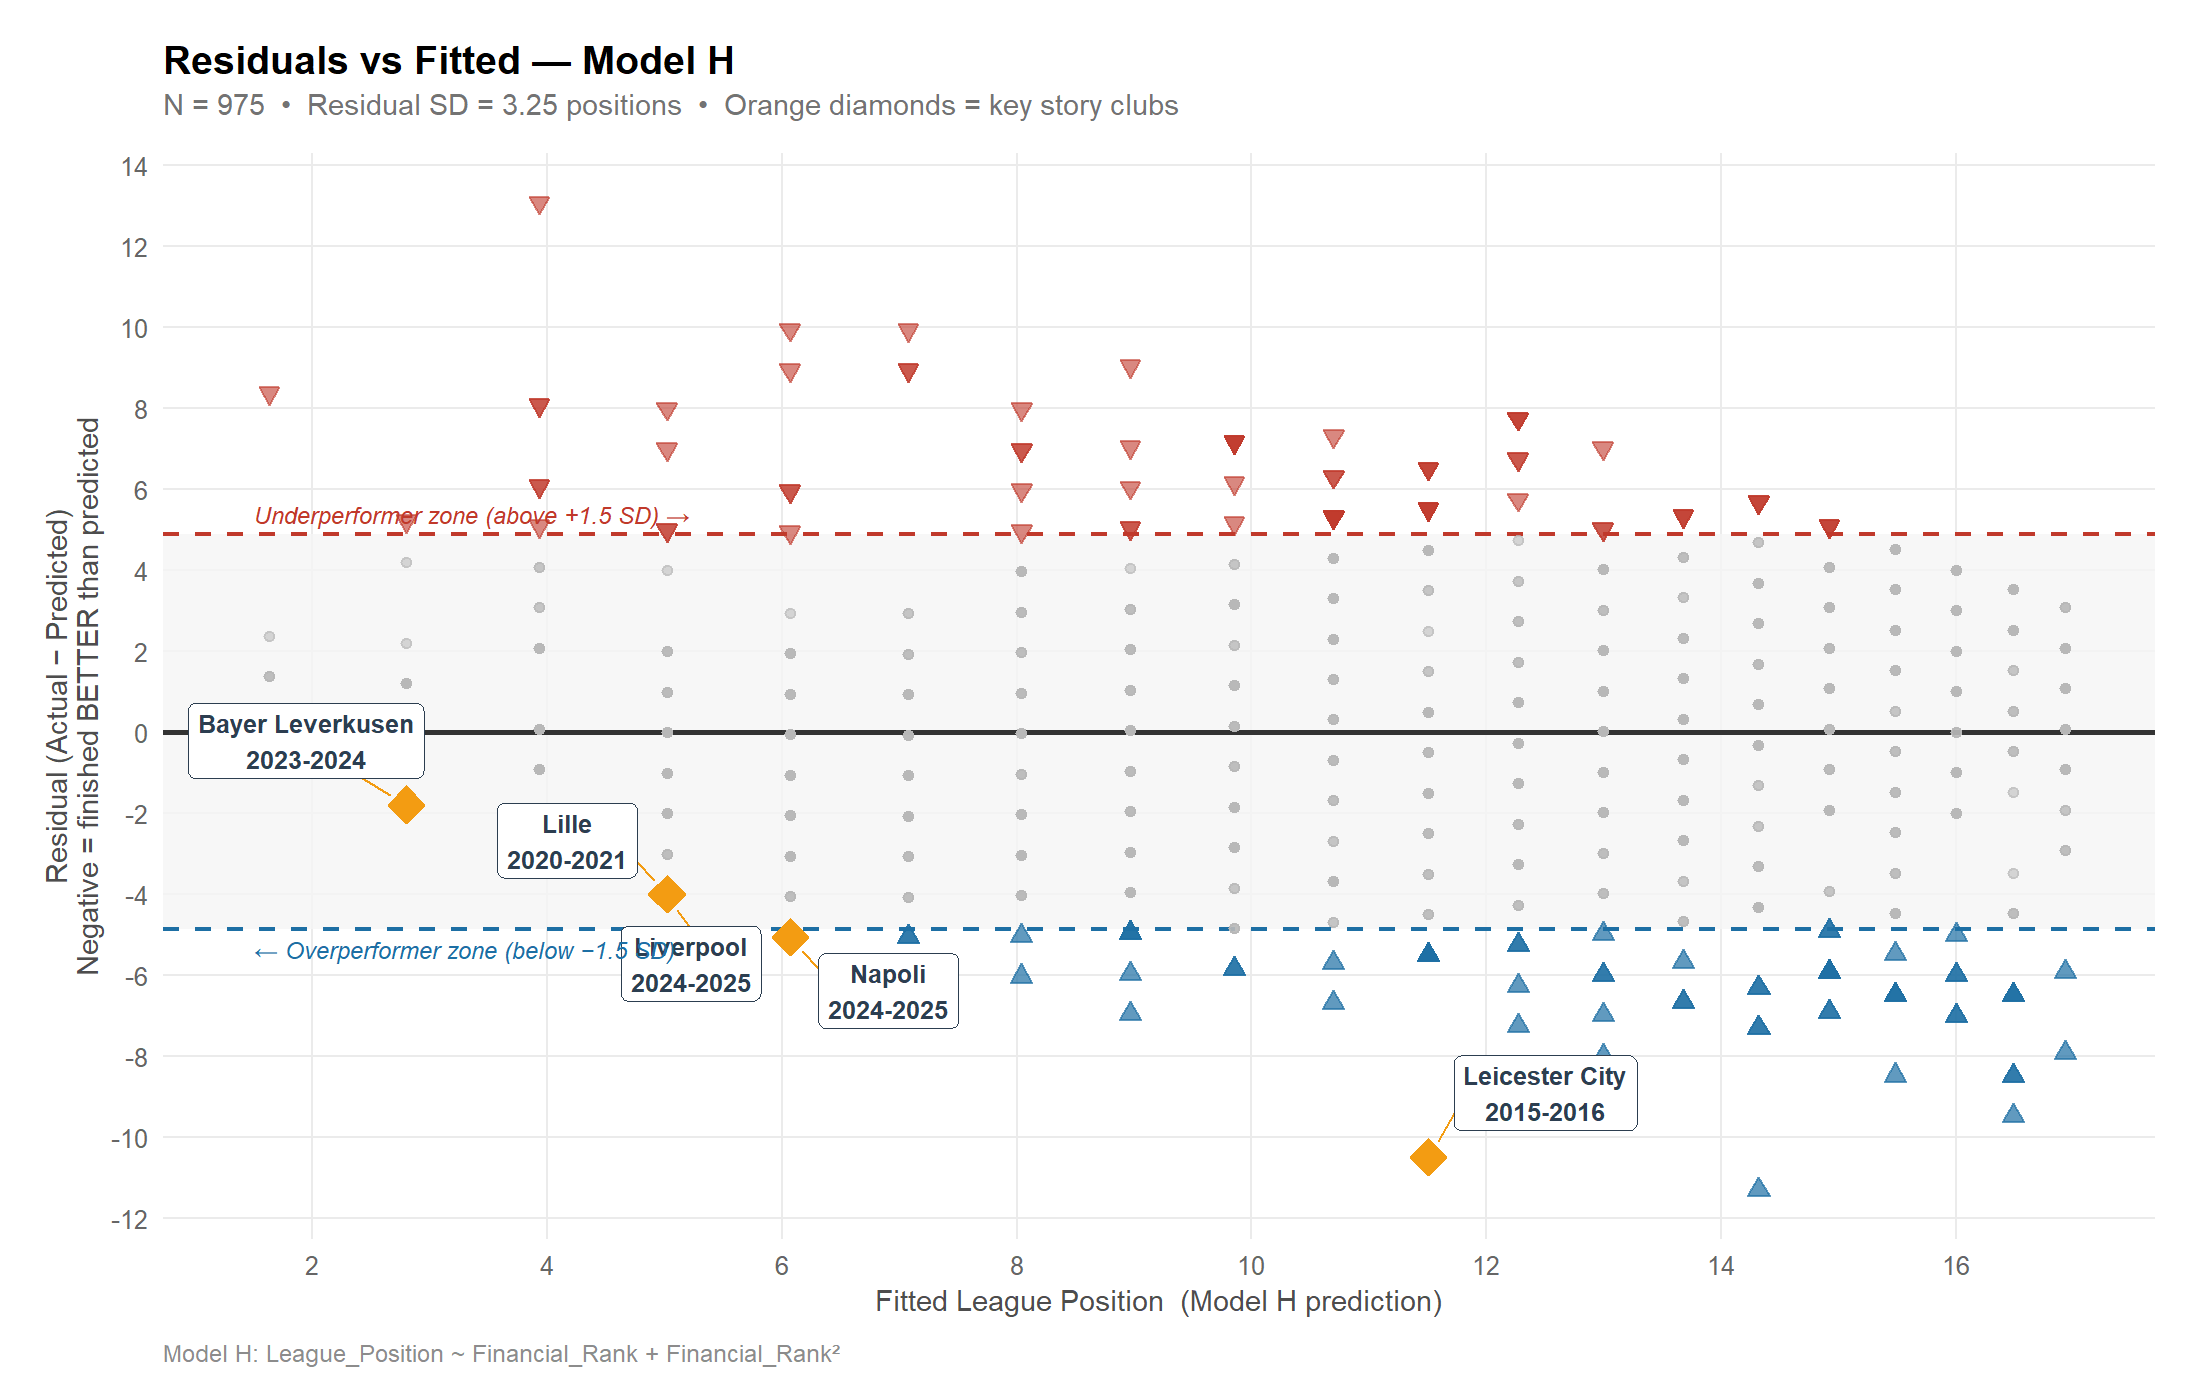
\includegraphics[width=0.95\linewidth, keepaspectratio]{28b_residual_plot_clean.png}
  \caption{Residuals vs.\ Fitted Values for Model~H. Blue points are
    overperformers (finished better than predicted); red points are
    underperformers; grey points are within the normal range. Dashed lines
    mark the $\pm 1.5$~SD outlier thresholds. Notable clubs are labelled.}
  \label{fig:resid}
\end{figure}

\subsection{Cook's Distance: Statistical Influence}

Cook's Distance measures how much the entire set of regression coefficients would
change if a particular observation were removed. The conventional threshold is
$4/N = 4/975 = 0.0041$.

\begin{figure}[H]
  \centering
  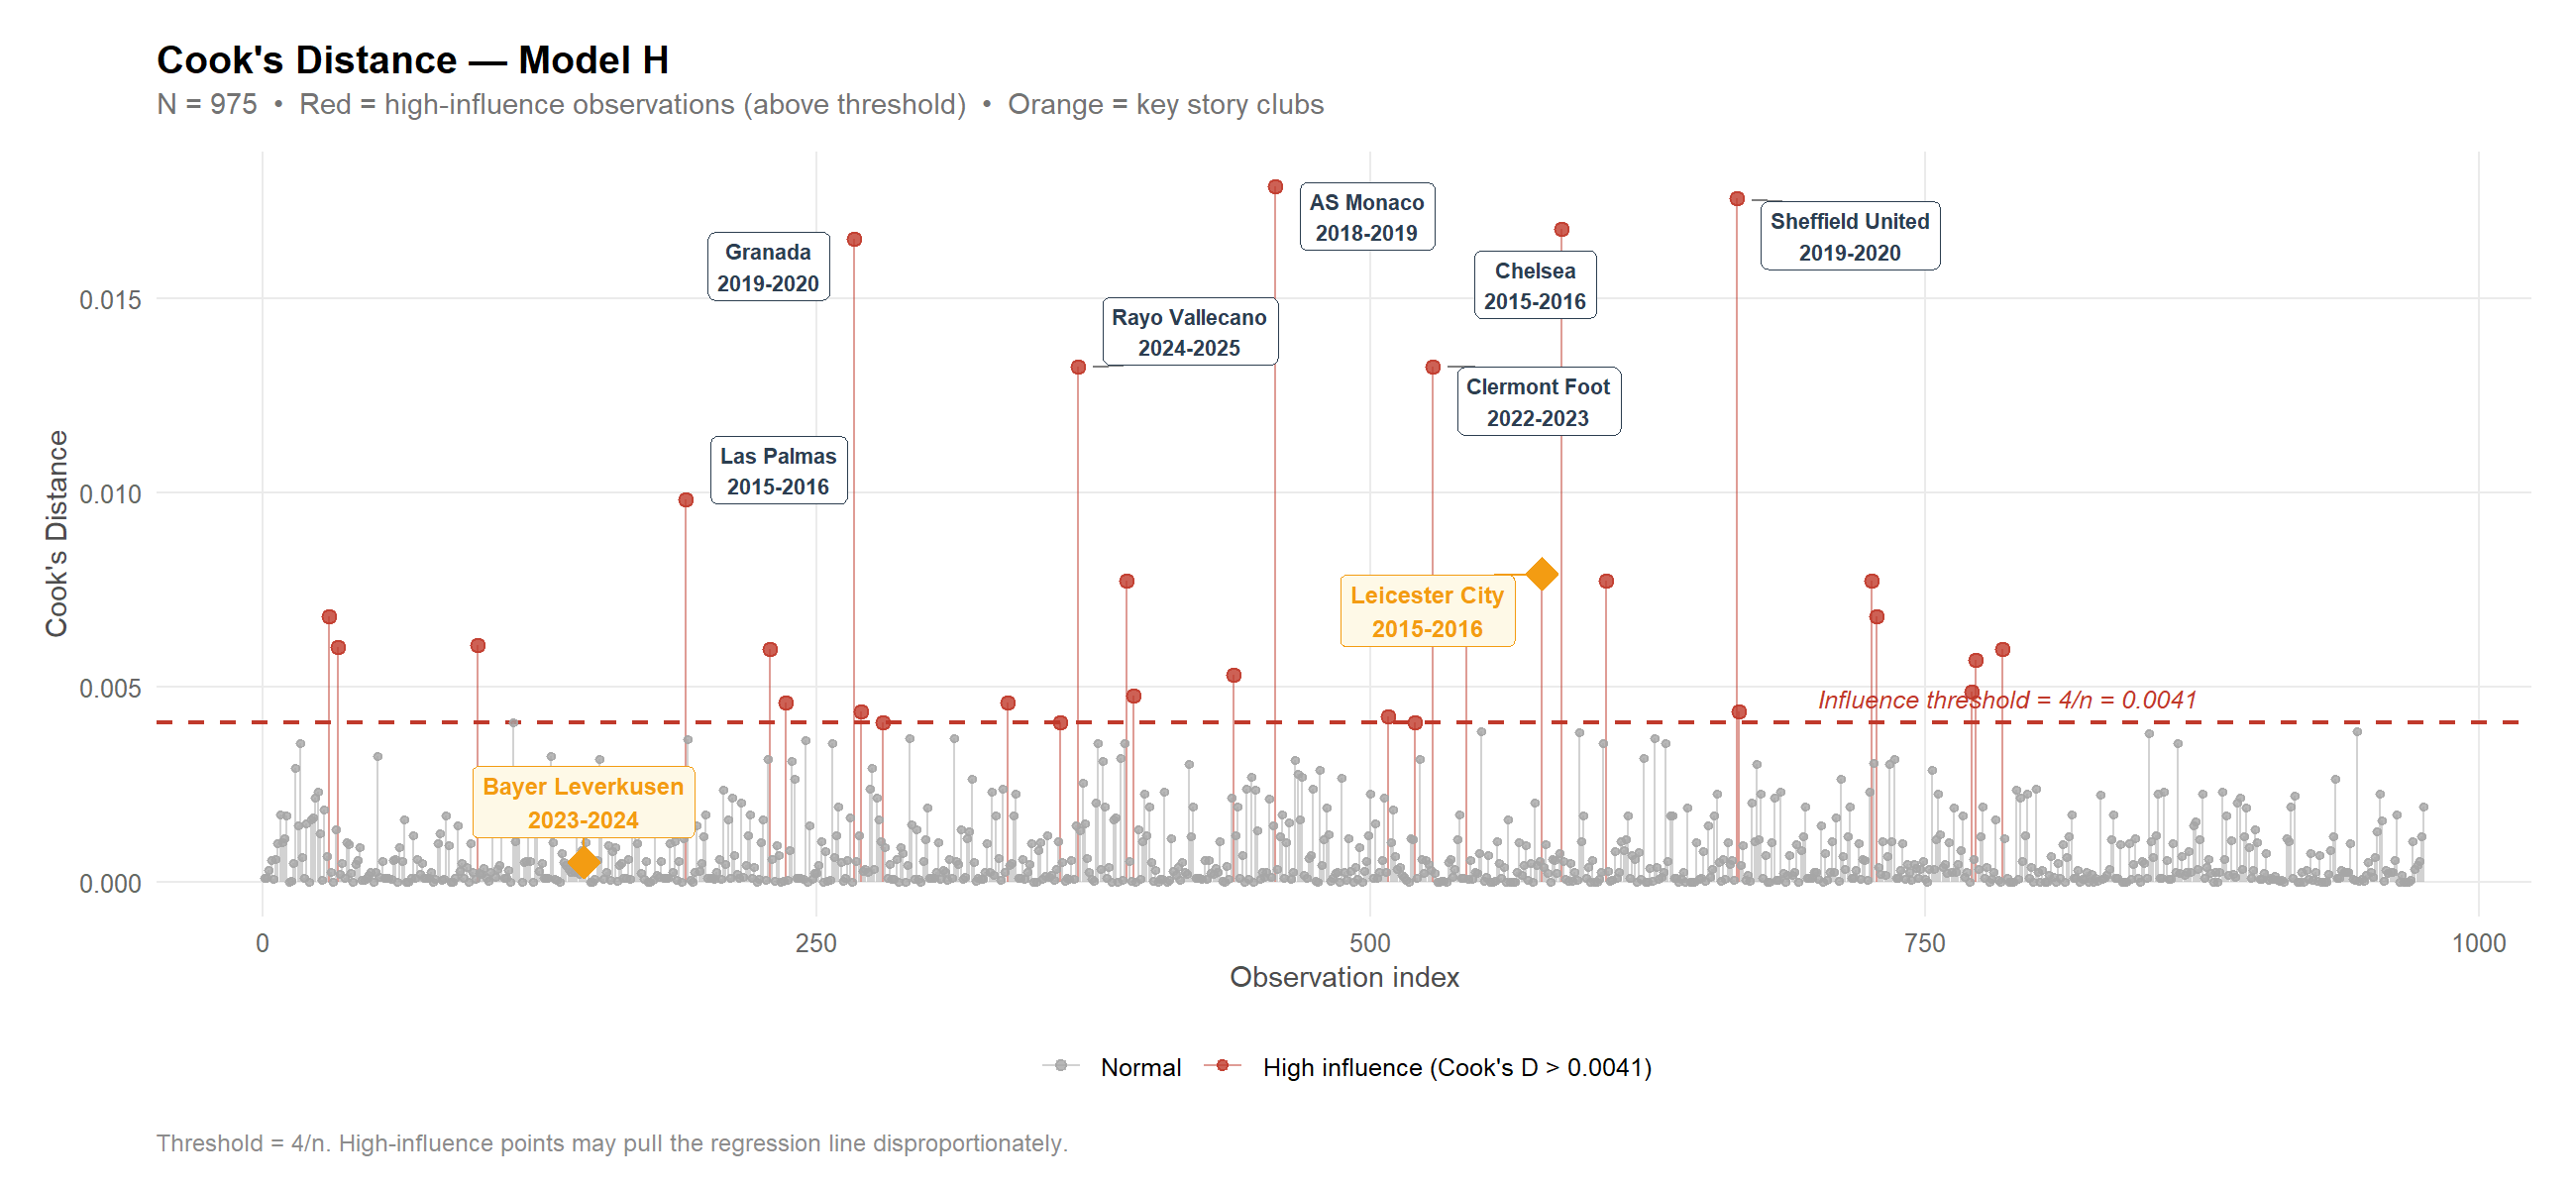
\includegraphics[width=0.95\linewidth, keepaspectratio]{29b_cooks_distance_clean.png}
  \caption{Cook's Distance for all 975 observations. The dashed red line marks
    the threshold $4/N = 0.0041$. Points above the line are statistically
    influential. The top entries are labelled by club name and season.}
  \label{fig:cooks}
\end{figure}

The most influential observation --- by a wide margin --- is Leicester City
2015--16. Their Cook's~$D = 0.187$, far above the threshold of 0.0041, confirming
this is not a data error but a statistically unprecedented event.

\subsection{Predicted vs.\ Actual: Selected Team-Seasons}

\begin{figure}[H]
  \centering
  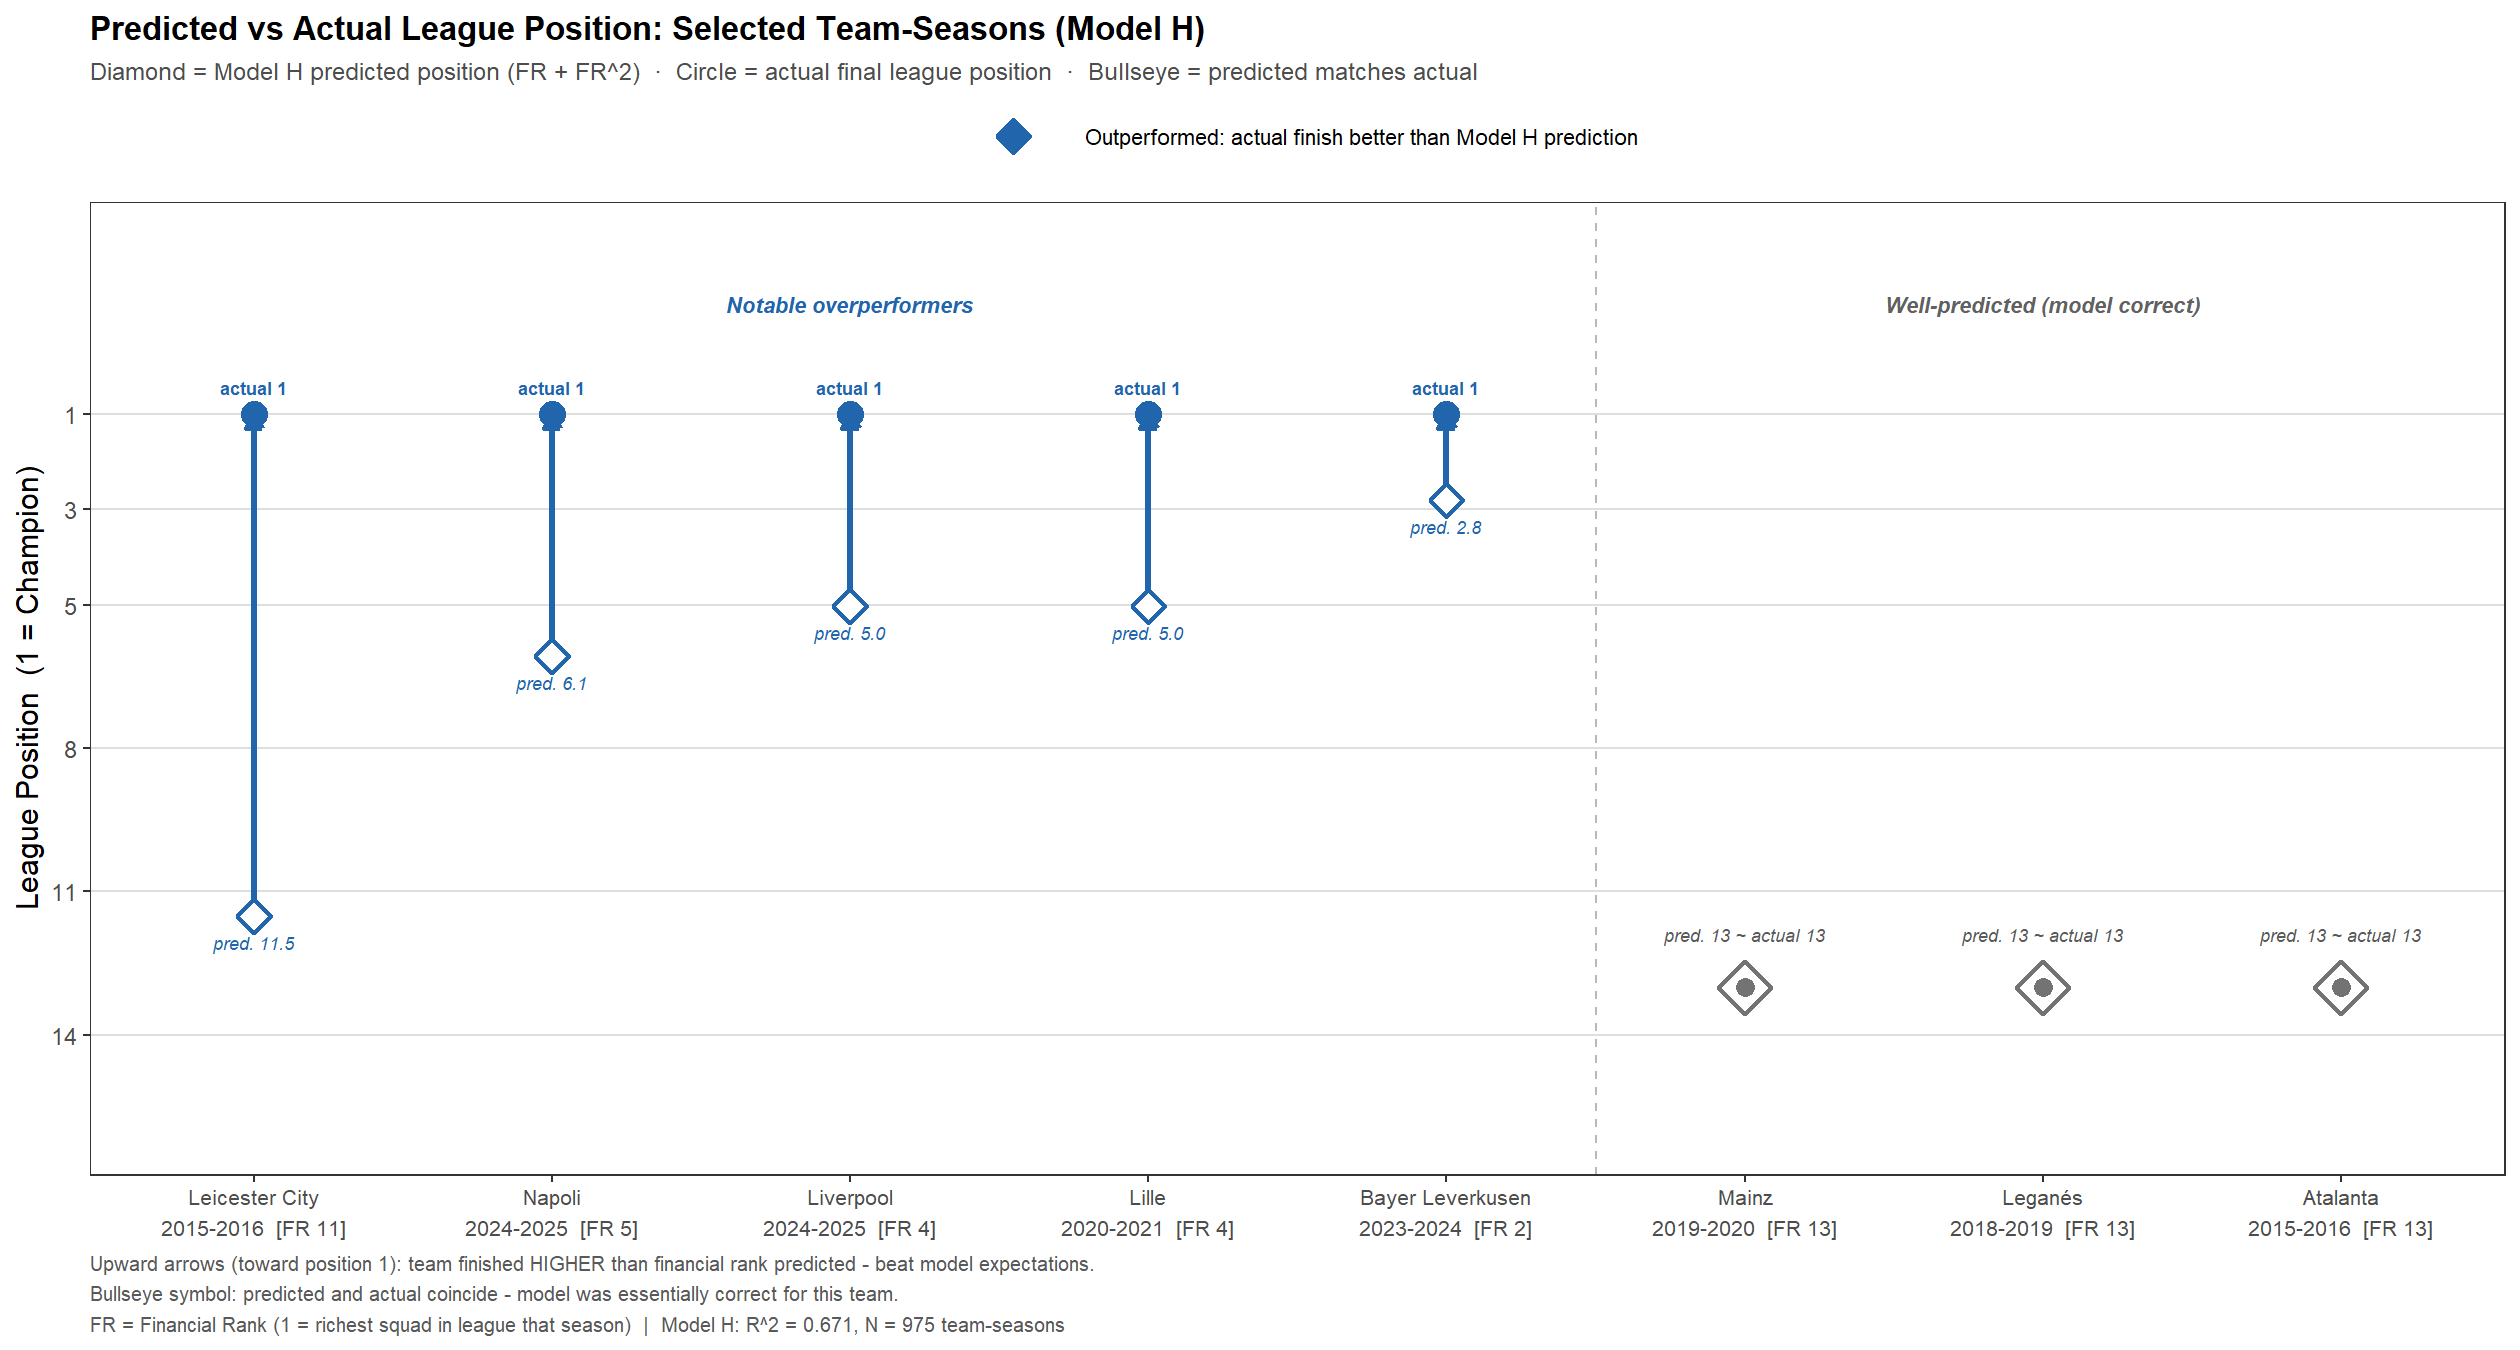
\includegraphics[width=\linewidth, keepaspectratio]{35_predicted_vs_actual_dumbbell.png}
  \caption{Predicted vs.\ actual league position for notable team-seasons (Model~H
    dumbbell chart). Diamond = Model~H predicted position;
    Circle = actual final position. Arrows indicate direction and magnitude of
    deviation. Bullseye symbols (right panel) show ``well-predicted'' contrast
    teams where the model was essentially correct. FR = Financial Rank.}
  \label{fig:dumbbell}
\end{figure}

Figure~\ref{fig:dumbbell} illustrates the residual analysis concretely. The five
featured overperformers all show large upward arrows (finishing far higher than
predicted). Leicester's arrow spans 10.5~positions --- the largest in the dataset.
The contrast teams on the right show perfect bullseye symbols, indicating the
model predicted their finish essentially exactly.

%% ===========================================================
\section{Step 5 --- The Exceptions: Cinderella Stories}
\label{sec:exceptions}
%% ===========================================================

\subsection{Champions from Outside the Financial Top Three}

Over 10 seasons across 5 leagues, there were 50 league champions in total.
Table~\ref{tab:surprisechamps} shows the financial breakdown.

\begin{table}[H]
  \centering
  \small
  \caption{Distribution of Financial Rank among the 50 league champions (2015--16 to 2024--25).}
  \label{tab:champfr}
  \begin{tabular}{c r r}
    \toprule
    \rowcolor{NavyBlue}
    \color{white}\textbf{Financial Rank} &
    \color{white}\textbf{Number of Champions} &
    \color{white}\textbf{Percentage} \\
    \midrule
    \rowcolor{RowB}
    \textbf{1} & \textbf{38} & \textbf{76\,\%} \\
    2 &  6 & 12\,\% \\
    3 &  2 &  4\,\% \\
    4 &  2 &  4\,\% \\
    5 &  1 &  2\,\% \\
    11 & 1 &  2\,\% \\
    \midrule
    \textbf{Total} & \textbf{50} & \textbf{100\,\%} \\
    \bottomrule
  \end{tabular}
\end{table}

\begin{figure}[H]
  \centering
  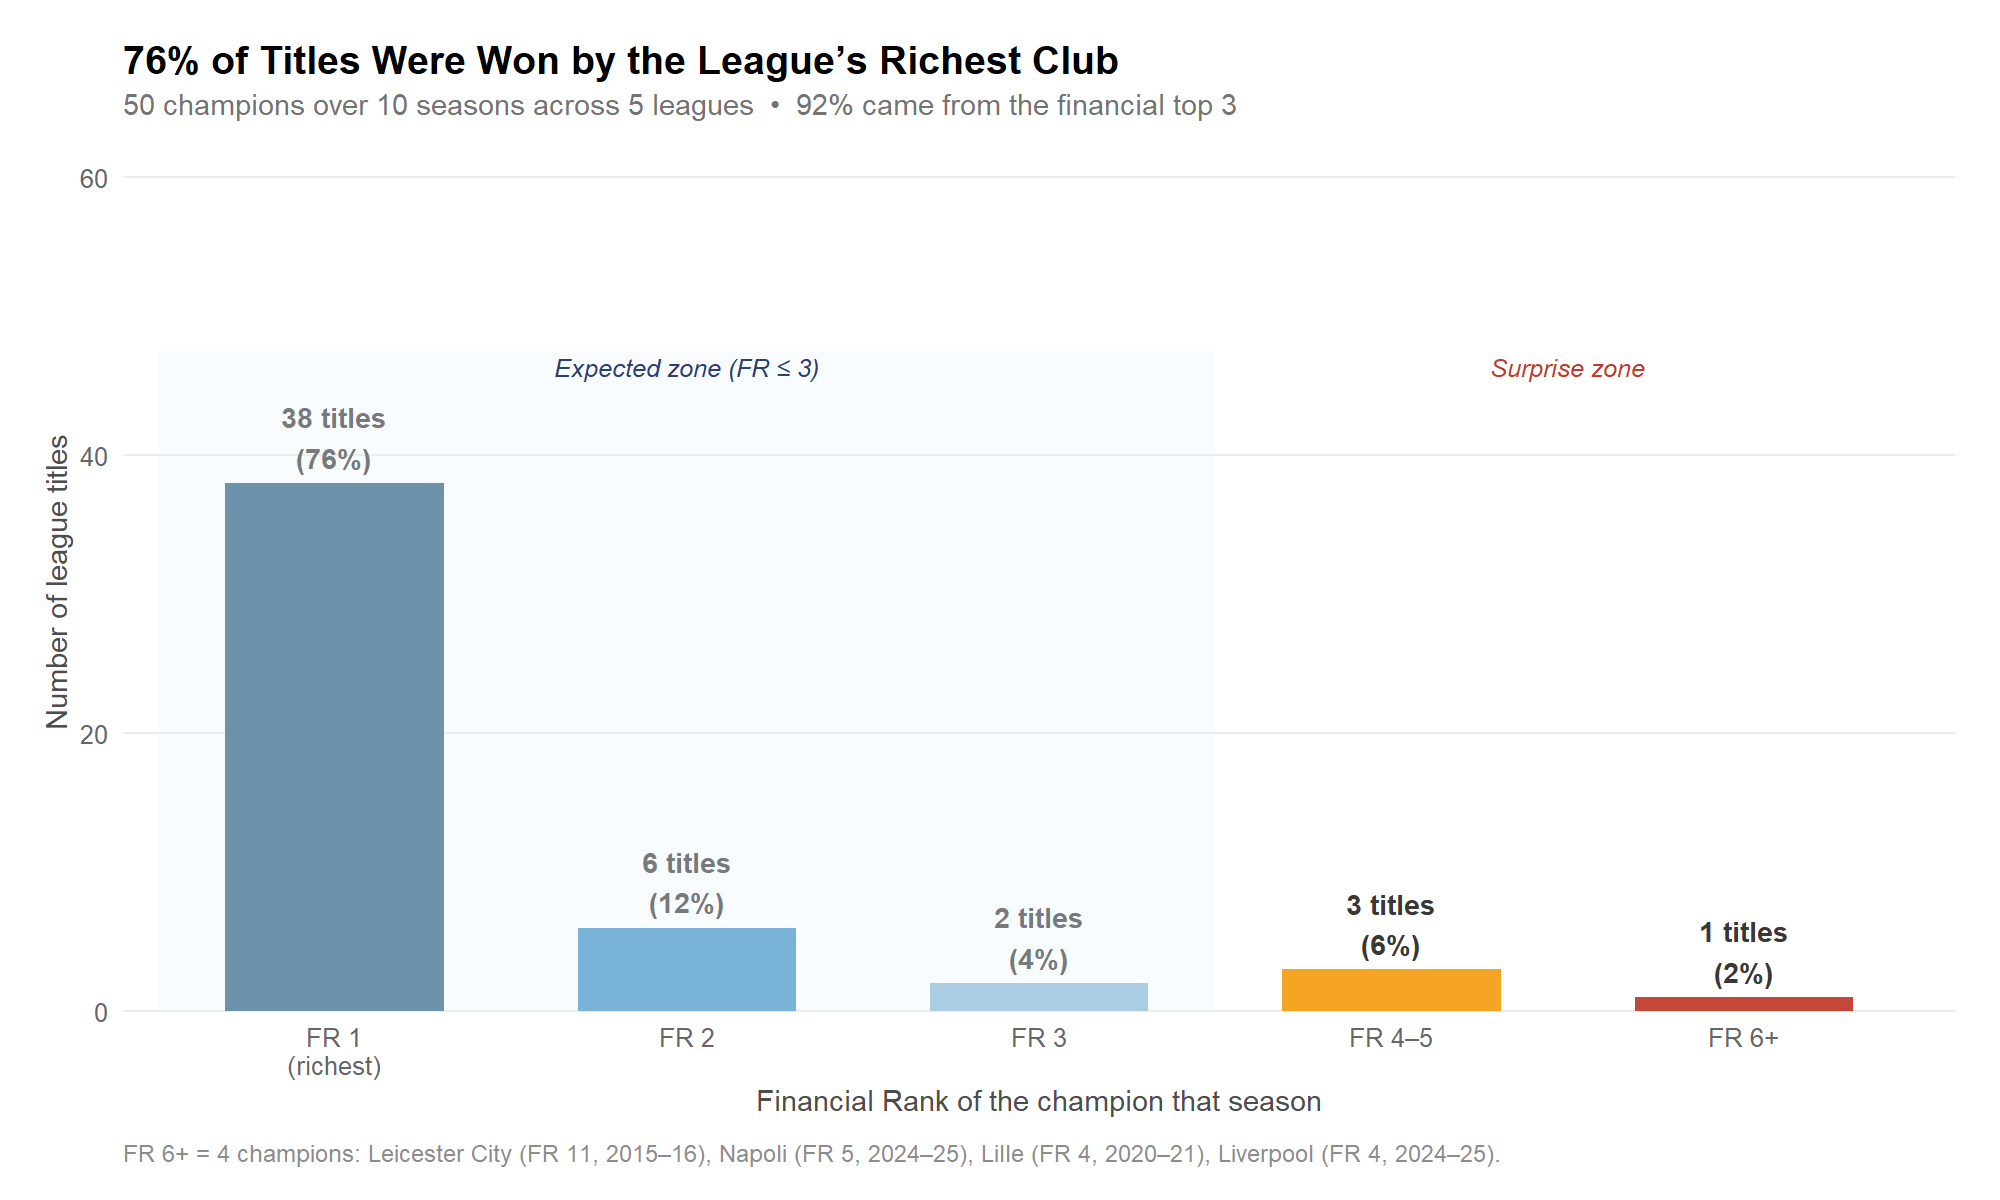
\includegraphics[width=0.88\linewidth, keepaspectratio]{34_champions_fr_dist.png}
  \caption{Distribution of Financial Rank among all 50 league champions across
    10 seasons and 5 leagues. The bar for FR\,=\,1 towers over all others ---
    38 of 50 titles (76\,\%) were won by the wealthiest club. Beyond FR\,=\,3,
    championship titles are extremely rare.}
  \label{fig:champfrdist}
\end{figure}

\begin{table}[H]
  \centering
  \small
  \caption{The 4 champions who won from outside the financial top 3 (FR\,>\,3).}
  \label{tab:surprisechamps}
  \begin{tabular}{l l l c r r r}
    \toprule
    \rowcolor{NavyBlue}
    \color{white}\textbf{League} &
    \color{white}\textbf{Season} &
    \color{white}\textbf{Club} &
    \color{white}\textbf{FR} &
    \color{white}\textbf{Value (M\EUR{})} &
    \color{white}\textbf{Predicted} &
    \color{white}\textbf{Residual} \\
    \midrule
    \rowcolor{RowC}
    \textbf{Premier League} & \textbf{2015--16} & \textbf{Leicester City}
      & \textbf{11} & \textbf{161.1} & \textbf{11.5} & \textbf{$-10.5$} \\
    Serie A   & 2024--25 & Napoli          &  5 & 500.5 &  6.1 & $-5.1$ \\
    \rowcolor{RowA}
    Ligue 1   & 2020--21 & Lille           &  4 & 323.2 &  5.0 & $-4.0$ \\
    Premier League & 2024--25 & Liverpool  &  4 & 950.9 &  5.0 & $-4.0$ \\
    \bottomrule
  \end{tabular}
  \medskip

  \noindent\small Note: Predicted = Model~H predicted position; Residual = Actual
  $-$ Predicted (negative = beat the model). Leicester is highlighted in red as the
  only genuine statistical outlier (residual $> 1.5$~SD from mean).
\end{table}

\begin{alertbox}
  \textbf{The sobering reality:} Only 4 of 50 champions (8\,\%) came from
  outside the financial top three. Of these 4 cases, three clubs (Napoli FR\,=\,5,
  Lille FR\,=\,4, Liverpool FR\,=\,4) were financially competitive --- only one or
  two steps outside the top tier. \textbf{Only Leicester City} (FR\,=\,11) is a
  genuine statistical outlier. The rest of the ``surprises'' are barely surprising
  when you examine their finances closely.
\end{alertbox}

\subsection{Leicester City 2015--16: A Closer Look}

\begin{table}[H]
  \centering
  \small
  \caption{Leicester City 2015--16 vs.\ Model~H expectations.}
  \label{tab:leicester}
  \begin{tabular}{l l}
    \toprule
    \rowcolor{NavyBlue}
    \color{white}\textbf{Metric} &
    \color{white}\textbf{Value} \\
    \midrule
    Financial Rank (Premier League, 2015--16)   & 11th (out of 20) \\
    Squad Market Value                           & \EUR{}161.1M \\
    \rowcolor{RowA}
    Model H: Predicted Position                 & \textbf{11.5} \\
    Actual Final Position                       & \textbf{1st (Champions)} \\
    \rowcolor{RowB}
    Residual                                    & \textbf{$-10.5$ positions} \\
    Residuals SD (all 975 obs.)                 & $\approx 3.25$ \\
    Residual in SD units                        & $\mathbf{-3.2\ \text{SD}}$ \\
    \rowcolor{RowA}
    Cook's Distance                             & 0.187 \\
    Cook's~$D$ Threshold ($4/N$)                & 0.0041 \\
    \bottomrule
  \end{tabular}
\end{table}

\begin{alertbox}
  \textbf{Quantifying the miracle:} Leicester's residual of $-10.5$~positions
  corresponds to \textbf{3.2~standard deviations} below the mean. In a normal
  distribution, an observation 3.2~SDs from the mean occurs with probability
  well below 0.1\,\%. Their Cook's Distance (0.187) is 46 times the threshold
  (0.0041), confirming it is a genuine, mathematically unprecedented event in
  this 10-season study. Importantly, removing Leicester from the dataset does
  \textbf{not} weaken our core finding --- if anything, it marginally
  \emph{increases} Model~H's $R^{2}$, showing the result is robust to this
  extraordinary case.
\end{alertbox}

%% ===========================================================
\section{Step 6 --- Is This Finding Reliable? Robustness Checks}
\label{sec:robustness}
%% ===========================================================

\subsection{Confirming the Quadratic Shape with Formal F-Tests}

We used nested F-tests to formally verify the quadratic specification and the
absence of meaningful cross-league or time-based variation.

\begin{table}[H]
  \centering
  \small
  \caption{Nested F-test results for Model~H specification checks.}
  \label{tab:ftests}
  \begin{tabular}{p{5.5cm} r r l p{4.0cm}}
    \toprule
    \rowcolor{NavyBlue}
    \color{white}\textbf{Comparison} &
    \color{white}\textbf{df} &
    \color{white}\textbf{$F$-statistic} &
    \color{white}\textbf{$p$-value} &
    \color{white}\textbf{Verdict} \\
    \midrule
    \rowcolor{RowB}
    Quadratic (FR+FR$^2$) vs.\ Linear (FR)
      & 1 & 31.71 & $< 0.001^{***}$
      & Quadratic term confirmed \\
    Interaction (FR$\times$League) vs.\ Additive
      & 4 & 1.17  & 0.324
      & Effect is league-uniform \\
    \rowcolor{RowA}
    Time-trend (FR$\times$Season) vs.\ Additive
      & 1 & 0.44  & 0.506
      & Effect is time-stable \\
    Cubic (FR+FR$^2$+FR$^3$) vs.\ Quadratic
      & 1 & 0.20  & 0.653
      & Cubic term not needed \\
    \bottomrule
  \end{tabular}
\end{table}

\begin{successbox}
  \textbf{All four robustness checks pass:}
  \begin{enumerate}[noitemsep]
    \item The quadratic term FR$^2$ is highly significant
          ($F_{1} = 31.71$, $p < 0.001$), confirming the non-linear shape is real.
    \item The interaction of FR with League is not significant ($F_{4} = 1.17$,
          $p = 0.324$), confirming the financial hierarchy works identically in
          all five leagues.
    \item There is no significant time trend ($F_{1} = 0.44$, $p = 0.506$),
          confirming the relationship has been stable from 2015--16 through 2024--25.
    \item The cubic term FR$^3$ is not significant ($F_{1} = 0.20$, $p = 0.653$),
          confirming Model~H (FR + FR$^2$) is the correct and sufficient specification.
  \end{enumerate}
\end{successbox}

\subsection{Time Stability: Has the Relationship Changed Over a Decade?}

\begin{figure}[H]
  \centering
  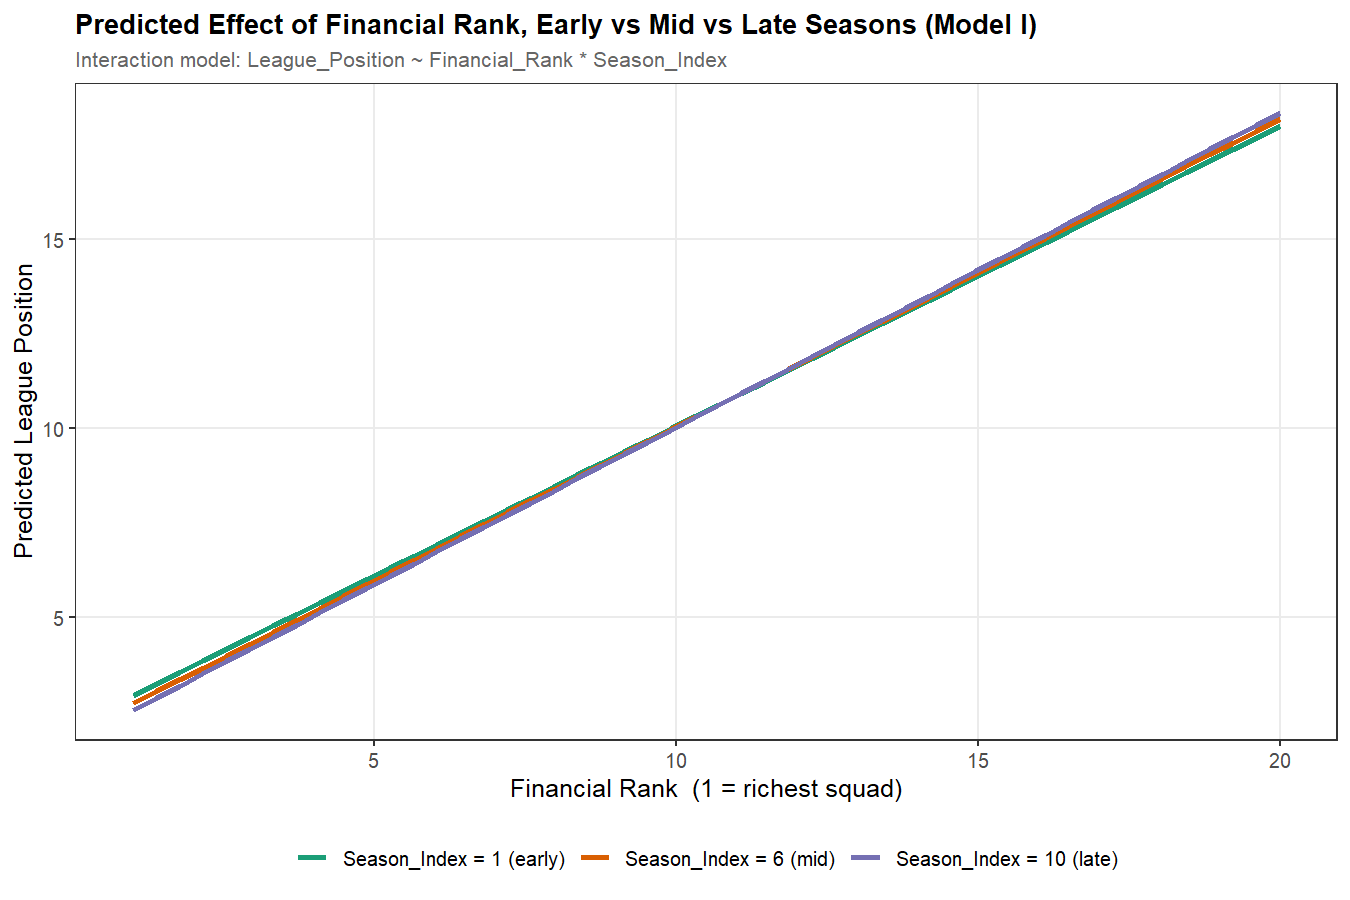
\includegraphics[width=0.88\linewidth, keepaspectratio]{23_time_trend_plot.png}
  \caption{The estimated effect of Financial Rank on League Position plotted
    across all 10 seasons (2015--16 to 2024--25). The flat trend line and wide
    confidence intervals confirm there is no significant time trend.}
  \label{fig:timetrend}
\end{figure}

The FR\,$\times$\,Season\_Index interaction coefficient is very close to zero and
statistically non-significant ($p = 0.506$). \textbf{The financial-position
relationship has neither strengthened nor weakened over the decade studied.} It
was as powerful in 2024--25 as it was in 2015--16.

\subsection{League-Interaction Test: Does the Effect Vary Across Leagues?}

\begin{figure}[H]
  \centering
  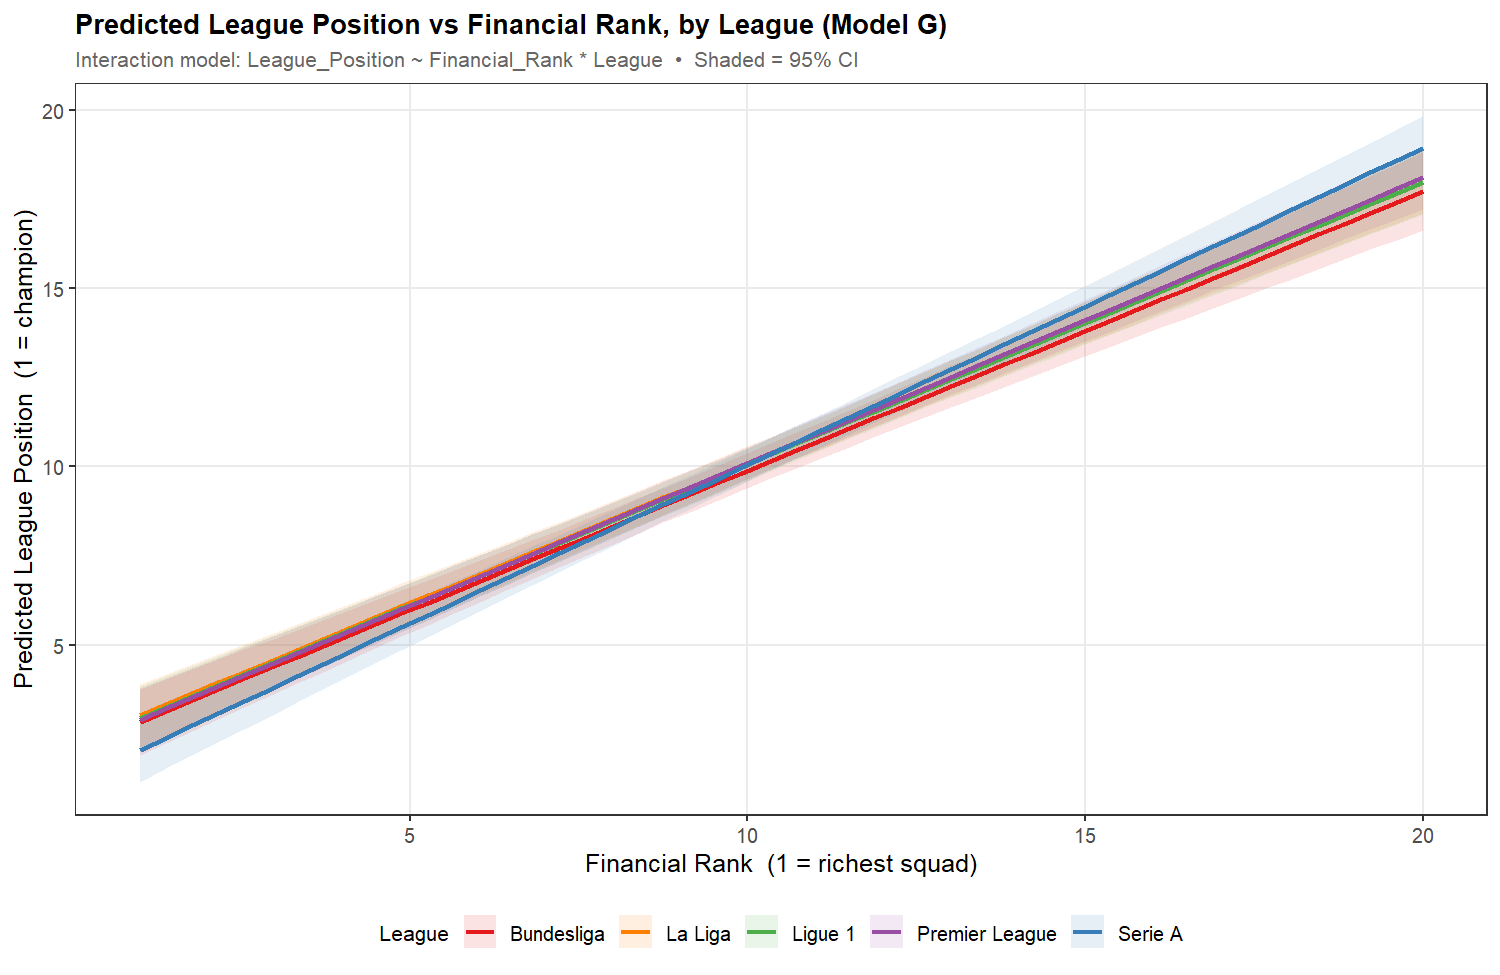
\includegraphics[width=0.88\linewidth, keepaspectratio]{19_interaction_slopes_by_league.png}
  \caption{Regression slopes (FR effect on league position) by individual league.
    The overlapping confidence intervals across all five leagues confirm the
    financial hierarchy operates identically in every league.}
  \label{fig:slopes}
\end{figure}

\subsection{Extended Model H4: Adding League and Season Controls}
\label{sec:modelh4}

We fit three extended variants of Model~H:
\begin{itemize}
  \item \textbf{H2:} FR + FR$^2$ + League (four league dummy variables)
  \item \textbf{H3:} FR + FR$^2$ + Season\_Index (linear time trend)
  \item \textbf{H4:} FR + FR$^2$ + League + Season\_Index (both controls)
\end{itemize}

\begin{table}[H]
  \centering
  \small
  \caption{Model~H family: adding League and Season controls.}
  \label{tab:h4comparison}
  \begin{tabular}{l l r r r r r}
    \toprule
    \rowcolor{NavyBlue}
    \color{white}\textbf{Model} &
    \color{white}\textbf{Formula} &
    \color{white}\textbf{N} &
    \color{white}\textbf{$R^{2}$} &
    \color{white}\textbf{Adj.~$R^{2}$} &
    \color{white}\textbf{AIC} &
    \color{white}\textbf{BIC} \\
    \midrule
    \rowcolor{RowB}
    \textbf{H}  & FR + FR$^{2}$                   & 975 & 0.6709 & 0.6703 & \textbf{5070.5} & 5090.1 \\
    H2 & FR + FR$^{2}$ + League          & 975 & 0.6714 & 0.6693 & 5077.3 & 5116.4 \\
    \rowcolor{RowA}
    H3 & FR + FR$^{2}$ + Season          & 975 & 0.6709 & 0.6699 & 5072.5 & 5096.9 \\
    H4 & FR + FR$^{2}$ + League + Season & 975 & 0.6714 & 0.6690 & 5079.3 & 5123.2 \\
    \bottomrule
  \end{tabular}
\end{table}

\begin{table}[H]
  \centering
  \small
  \caption{Nested F-tests: extending Model~H with League and Season controls.}
  \label{tab:h4ftests}
  \begin{tabular}{p{5.5cm} r r l}
    \toprule
    \rowcolor{NavyBlue}
    \color{white}\textbf{Comparison} &
    \color{white}\textbf{df} &
    \color{white}\textbf{$F$-statistic} &
    \color{white}\textbf{$p$-value} \\
    \midrule
    H2 vs.\ H: Adding League FE       & 4 & 0.304 & 0.876 \\
    \rowcolor{RowA}
    H3 vs.\ H: Adding Season\_Index   & 1 & 0.023 & 0.880 \\
    H4 vs.\ H: League + Season (joint) & 5 & 0.247 & 0.941 \\
    \rowcolor{RowA}
    H4 vs.\ H2: Season beyond League  & 1 & 0.023 & 0.879 \\
    H4 vs.\ H3: League beyond Season  & 4 & 0.303 & 0.876 \\
    \bottomrule
  \end{tabular}
\end{table}

Model~H4 achieves $R^2 = 0.6714$ and AIC = 5079.3, compared to Model~H's
$R^2 = 0.6709$ and AIC = 5070.5. Model~H wins on AIC by 8.75~points; the joint
$F$-test yields $F(5) = 0.247$, $p = 0.941$ --- not significant at any conventional
level. \textbf{Conclusion: Model~H (FR + FR$^2$) is the correct and sufficient
specification.} Adding league intercepts or a time trend does not improve fit.

\subsection{Heteroskedasticity Check}

The Breusch--Pagan test detects significant heteroskedasticity in the residuals
($p < 0.001$). We verified that re-estimating the model with HC1
heteroskedasticity-robust standard errors leaves the main conclusions unchanged:
Financial Rank remains highly significant ($z > 15$, $p < 0.001$), and the
percentage changes in standard errors are modest. Our findings are not sensitive
to non-constant residual variance.

%% ===========================================================
\section{Conclusions}
%% ===========================================================

\subsection{Summary of Findings}

\begin{findingbox}
  \textbf{Finding 1 --- Money very strongly predicts where clubs finish.}
  The Pearson correlation is $r = 0.813$ (Spearman $\rho = 0.814$), both
  $p < 0.001$ across all 975 team-seasons. Model~H (quadratic in FR)
  explains $R^{2} = 0.671$ --- nearly two-thirds of all variation in final
  standings --- using nothing but a club's within-league wealth rank.
\end{findingbox}

\begin{findingbox}
  \textbf{Finding 2 --- The relationship is non-linear: diminishing returns at the bottom.}
  Adding FR$^2$ significantly improves model fit ($F_{1} = 31.71$, $p < 0.001$).
  The marginal positional penalty of dropping one rank is largest at the top of
  the financial hierarchy ($\approx 1.19$ positions per rank at FR\,1\,\textrightarrow\,2)
  and shrinks at the bottom ($\approx 0.63$ positions at FR\,15\,\textrightarrow\,16).
  In plain language: the gap between the richest and second-richest club is much
  larger than the gap between the 15th and 16th richest.
\end{findingbox}

\begin{findingbox}
  \textbf{Finding 3 --- The effect is the same in every league and has not changed over time.}
  The FR\,$\times$\,League interaction is not significant ($F_{4} = 1.17$,
  $p = 0.324$): the financial hierarchy operates identically in Germany, Spain,
  France, England, and Italy. The FR\,$\times$\,Season time trend is also not
  significant ($F_{1} = 0.44$, $p = 0.506$): the relationship has been equally
  strong throughout 2015--16 to 2024--25.
\end{findingbox}

\begin{alertbox}
  \textbf{Finding 4 --- Exceptions exist, but only one is truly extraordinary.}
  Of 50 league titles across the decade, only 4 were won by clubs outside the
  financial top three. Three of those four (Napoli FR\,=\,5, Lille FR\,=\,4,
  Liverpool FR\,=\,4) were at most one or two steps outside the expected zone.
  Only \textbf{Leicester City 2015--16} --- FR\,=\,11, predicted 11th, actually
  champions --- is a genuine statistical outlier ($-3.2$~SD, Cook's~$D = 0.187$).
\end{alertbox}

\subsection{Limitations and Future Directions}

\begin{table}[H]
  \centering
  \small
  \caption{Study limitations and suggested future extensions.}
  \label{tab:limitations}
  \begin{tabular}{p{2.8cm} p{5.8cm} p{5.4cm}}
    \toprule
    \rowcolor{NavyBlue}
    \color{white}\textbf{Limitation} &
    \color{white}\textbf{Issue} &
    \color{white}\textbf{Potential Fix} \\
    \midrule
    \textbf{Market value as quality proxy}
      & Transfermarkt valuations may lag actual squad quality; subjective editor estimates
      & Use wage bill data; cross-validate with Opta squad ratings \\
    \rowcolor{RowA}
    \textbf{No managerial quality}
      & Exceptional coaches (e.g., Ranieri at Leicester) are not captured in the model
      & Add manager tenure, prior record, or a coaching quality index \\
    \textbf{No injury data}
      & Injury crises can dramatically alter a squad's effective quality mid-season
      & Incorporate injury-adjusted squad value (weighted by availability) \\
    \rowcolor{RowA}
    \textbf{Panel structure ignored}
      & Teams appear in multiple seasons; correlated errors across seasons are unmodelled
      & Fixed-effects panel model or clustered standard errors at the team level \\
    \textbf{Top divisions only}
      & Results may not generalise to lower divisions or smaller national leagues
      & Replicate in Eredivisie, Championship, or Scottish Premiership \\
    \bottomrule
  \end{tabular}
\end{table}

%% ===========================================================
%% APPENDICES
%% ===========================================================
\appendix

\section{Full Coefficient Table (Models A--E)}
\label{app:coeftable}

\begin{table}[H]
  \centering
  \small
  \caption{Full regression coefficient table (Models A--E). $^{***}$ $p<0.001$;
    $^{**}$ $p<0.01$; $^*$ $p<0.05$.}
  \label{tab:fullcoefs}
  \begin{tabular}{l l r r r l}
    \toprule
    \rowcolor{NavyBlue}
    \color{white}\textbf{Model} &
    \color{white}\textbf{Term} &
    \color{white}\textbf{Estimate} &
    \color{white}\textbf{Std.\ Error} &
    \color{white}\textbf{$t$/$z$} &
    \color{white}\textbf{$p$-value} \\
    \midrule
    \multirow{2}{*}{A} & Intercept & 1.930 & 0.219 & 8.81 & $< 0.001^{***}$ \\
                       & Financial\_Rank & 0.812 & 0.019 & 43.48 & $< 0.001^{***}$ \\
    \midrule
    \rowcolor{RowA}
    \multirow{2}{*}{C} & Intercept & 2.891 & 0.254 & 11.38 & $< 0.001^{***}$ \\
    \rowcolor{RowA}
                       & Log(MV) & $-5.026$ & 0.151 & $-33.30$ & $< 0.001^{***}$ \\
    \midrule
    \multirow{3}{*}{H} & Intercept & 0.419 & 0.344 & 1.22 & 0.224 \\
                       & Financial\_Rank & 1.231 & 0.077 & 16.08 & $< 0.001^{***}$ \\
                       & FR$^{2}$ & $-0.0202$ & 0.0036 & $-5.63$ & $< 0.001^{***}$ \\
    \midrule
    \rowcolor{RowA}
    \multirow{2}{*}{E\,(Logit)} & Intercept & 1.642 & 0.403 & 4.07 & $< 0.001^{***}$ \\
    \rowcolor{RowA}
                       & Financial\_Rank & $-1.298$ & 0.190 & $-6.83$ & $< 0.001^{***}$ \\
    \bottomrule
  \end{tabular}
  \medskip

  \noindent\small Models B, D, G contain league fixed effects and season terms.
  Full tables available upon request from the project repository.
\end{table}

\section{All League Champions: Ranked by Residual}
\label{app:champions}

Table~\ref{tab:allchamps} lists all 50 league champions with their Financial Rank
and Model~H residual, sorted from greatest over-performance (most negative
residual) to least.

\begin{longtable}{l l l c r r}
  \caption{All 50 league champions (2015--16 to 2024--25), ranked by Model~H residual.
    Negative residual = finished better than predicted.}
  \label{tab:allchamps} \\
  \toprule
  \rowcolor{NavyBlue}
  \color{white}\textbf{League} &
  \color{white}\textbf{Season} &
  \color{white}\textbf{Club} &
  \color{white}\textbf{FR} &
  \color{white}\textbf{Predicted} &
  \color{white}\textbf{Residual} \\
  \midrule
  \endfirsthead
  \multicolumn{6}{c}{\small\textit{(continued from previous page)}} \\
  \toprule
  \rowcolor{NavyBlue}
  \color{white}\textbf{League} &
  \color{white}\textbf{Season} &
  \color{white}\textbf{Club} &
  \color{white}\textbf{FR} &
  \color{white}\textbf{Predicted} &
  \color{white}\textbf{Residual} \\
  \midrule
  \endhead
  \midrule
  \multicolumn{6}{r}{\small\textit{continued on next page}} \\
  \endfoot
  \bottomrule
  \endlastfoot
  \rowcolor{RowC}
  Premier League & 2015--16 & \textbf{Leicester City}  & 11 & 11.5 & $-10.5$ \\
  Serie A        & 2024--25 & Napoli                   &  5 &  6.1 & $-5.1$ \\
  Ligue 1        & 2020--21 & Lille                    &  4 &  5.0 & $-4.0$ \\
  Premier League & 2024--25 & Liverpool                &  4 &  5.0 & $-4.0$ \\
  La Liga        & 2020--21 & Atlético Madrid          &  3 &  3.9 & $-2.9$ \\
  Serie A        & 2021--22 & AC Milan                 &  3 &  3.9 & $-2.9$ \\
  Bundesliga     & 2023--24 & Bayer Leverkusen         &  2 &  2.8 & $-1.8$ \\
  La Liga        & 2019--20 & Real Madrid              &  2 &  2.8 & $-1.8$ \\
  La Liga        & 2022--23 & Barcelona                &  2 &  2.8 & $-1.8$ \\
  La Liga        & 2024--25 & Barcelona                &  2 &  2.8 & $-1.8$ \\
  Ligue 1        & 2016--17 & AS Monaco                &  2 &  2.8 & $-1.8$ \\
  Premier League & 2019--20 & Liverpool                &  2 &  2.8 & $-1.8$ \\
  Bundesliga     & 2015--16 & Bayern Munich            &  1 &  1.6 & $-0.6$ \\
  Bundesliga     & 2016--17 & Bayern Munich            &  1 &  1.6 & $-0.6$ \\
  Bundesliga     & 2017--18 & Bayern Munich            &  1 &  1.6 & $-0.6$ \\
  Bundesliga     & 2018--19 & Bayern Munich            &  1 &  1.6 & $-0.6$ \\
  Bundesliga     & 2019--20 & Bayern Munich            &  1 &  1.6 & $-0.6$ \\
  Bundesliga     & 2020--21 & Bayern Munich            &  1 &  1.6 & $-0.6$ \\
  Bundesliga     & 2021--22 & Bayern Munich            &  1 &  1.6 & $-0.6$ \\
  Bundesliga     & 2022--23 & Bayern Munich            &  1 &  1.6 & $-0.6$ \\
  Bundesliga     & 2024--25 & Bayern Munich            &  1 &  1.6 & $-0.6$ \\
  La Liga        & 2015--16 & Barcelona                &  1 &  1.6 & $-0.6$ \\
  La Liga        & 2016--17 & Real Madrid              &  1 &  1.6 & $-0.6$ \\
  La Liga        & 2017--18 & Barcelona                &  1 &  1.6 & $-0.6$ \\
  La Liga        & 2018--19 & Barcelona                &  1 &  1.6 & $-0.6$ \\
  La Liga        & 2021--22 & Real Madrid              &  1 &  1.6 & $-0.6$ \\
  La Liga        & 2023--24 & Real Madrid              &  1 &  1.6 & $-0.6$ \\
  Ligue 1        & 2015--16 & Paris Saint-Germain      &  1 &  1.6 & $-0.6$ \\
  Ligue 1        & 2017--18 & Paris Saint-Germain      &  1 &  1.6 & $-0.6$ \\
  Ligue 1        & 2018--19 & Paris Saint-Germain      &  1 &  1.6 & $-0.6$ \\
  Ligue 1        & 2019--20 & Paris Saint-Germain      &  1 &  1.6 & $-0.6$ \\
  Ligue 1        & 2021--22 & Paris Saint-Germain      &  1 &  1.6 & $-0.6$ \\
  Ligue 1        & 2022--23 & Paris Saint-Germain      &  1 &  1.6 & $-0.6$ \\
  Ligue 1        & 2023--24 & Paris Saint-Germain      &  1 &  1.6 & $-0.6$ \\
  Ligue 1        & 2024--25 & Paris Saint-Germain      &  1 &  1.6 & $-0.6$ \\
  Premier League & 2016--17 & Chelsea                  &  1 &  1.6 & $-0.6$ \\
  Premier League & 2017--18 & Manchester City          &  1 &  1.6 & $-0.6$ \\
  Premier League & 2018--19 & Manchester City          &  1 &  1.6 & $-0.6$ \\
  Premier League & 2020--21 & Manchester City          &  1 &  1.6 & $-0.6$ \\
  Premier League & 2021--22 & Manchester City          &  1 &  1.6 & $-0.6$ \\
  Premier League & 2022--23 & Manchester City          &  1 &  1.6 & $-0.6$ \\
  Premier League & 2023--24 & Manchester City          &  1 &  1.6 & $-0.6$ \\
  Serie A        & 2015--16 & Juventus                 &  1 &  1.6 & $-0.6$ \\
  Serie A        & 2016--17 & Juventus                 &  1 &  1.6 & $-0.6$ \\
  Serie A        & 2017--18 & Juventus                 &  1 &  1.6 & $-0.6$ \\
  Serie A        & 2018--19 & Juventus                 &  1 &  1.6 & $-0.6$ \\
  Serie A        & 2019--20 & Juventus                 &  1 &  1.6 & $-0.6$ \\
  Serie A        & 2020--21 & Internazionale           &  1 &  1.6 & $-0.6$ \\
  Serie A        & 2022--23 & Napoli                   &  1 &  1.6 & $-0.6$ \\
  Serie A        & 2023--24 & Internazionale           &  1 &  1.6 & $-0.6$ \\
\end{longtable}

\section{R Code Excerpts}
\label{app:code}

\textbf{Data loading and model setup:}
\begin{verbatim}
df <- read_csv("data/merged/master_dataset.csv") |>
  filter(!is.na(League_Position), !is.na(Financial_Rank)) |>
  mutate(League = factor(League, levels = league_order),
         Champion_bin = as.integer(
           tolower(Champion) %in% c("yes","true","1")))

modH <- lm(League_Position ~ Financial_Rank + I(Financial_Rank^2), data = df)
modE <- glm(Champion_bin ~ Financial_Rank, data = df, family = binomial())
\end{verbatim}

\textbf{Residual analysis and outlier flagging:}
\begin{verbatim}
aug_H <- augment(modH, data = df) |>
  rename(Fitted_H = .fitted, Residual_H = .resid, CooksD = .cooksd)

resid_sd <- sd(aug_H$Residual_H, na.rm = TRUE)

aug_H <- aug_H |>
  mutate(Outlier_Flag = case_when(
    Residual_H < -1.5 * resid_sd ~ "Overperformer",
    Residual_H >  1.5 * resid_sd ~ "Underperformer",
    TRUE                          ~ "Normal"))
\end{verbatim}

\textbf{Key analysis scripts:}

\begin{center}
\small
\begin{tabular}{ll}
  \toprule
  Script & Purpose \\
  \midrule
  \texttt{RScripts/01\_scrape\_ESPN\_standings.R}           & Download league standings \\
  \texttt{RScripts/02\_scrape\_transfermarkt\_market\_values.R} & Download squad market values \\
  \texttt{RScripts/03\_compute\_financial\_rank.R}          & Assign within-league Financial Rank \\
  \texttt{RScripts/04\_merge\_standings\_and\_market\_values.R} & Build master dataset \\
  \texttt{RScripts/05\_analysis\_and\_regression.R}         & Core OLS and logit models \\
  \texttt{RScripts/05b\_extended\_regression.R}             & Robustness checks \\
  \texttt{RScripts/06\_residuals\_and\_outliers.R}          & Residual analysis, Cook's Distance \\
  \texttt{RScripts/07\_beautiful\_charts.R}                 & Publication-quality visualisations \\
  \bottomrule
\end{tabular}
\end{center}

%% ===========================================================
\section{Session and Reproducibility Information}
\label{app:session}
%% ===========================================================

\begin{center}
\small
\begin{tabular}{ll}
  \toprule
  \textbf{Item} & \textbf{Value} \\
  \midrule
  R version          & 4.4.x \\
  Platform           & Windows 11 Enterprise \\
  Analysis date      & June 2026 \\
  Key packages       & dplyr, ggplot2, broom, kableExtra, ggrepel, sandwich \\
  Data sources       & ESPN FC (standings), Transfermarkt (squad values) \\
  \bottomrule
\end{tabular}
\end{center}

%% ===========================================================
\begin{thebibliography}{9}

\bibitem{Szymanski1999}
Szymanski, S., \& Kuypers, T. (1999).
\textit{Winners \& Losers: The Business Strategy of Football}.
Viking.

\bibitem{Frick2007}
Frick, B. (2007).
The football players' labor market: Empirical evidence from the major
European leagues.
\textit{Scottish Journal of Political Economy}, 54(3), 422--446.

\bibitem{Dobson2001}
Dobson, S., \& Goddard, J. (2001).
\textit{The Economics of Football}.
Cambridge University Press.

\bibitem{Deloitte2025}
Deloitte Sports Business Group. (2025).
\textit{Annual Review of Football Finance}.
Deloitte.

\end{thebibliography}

\vfill
\noindent\small
\textit{Report compiled in \LaTeX{}. Data: ESPN FC (league standings),
Transfermarkt (squad market values). All analysis scripts are in the project
\texttt{RScripts/} directory. Contact:
\href{mailto:mdmuktadir0611@gmail.com}{mdmuktadir0611@gmail.com}}

\end{document}
